\documentclass[a4paper,12pt]{article}
\usepackage[top=2cm, bottom=2cm, left=1.5cm, right=1.5cm]{geometry}
\usepackage{amsmath}
\usepackage{multicol}
\usepackage{graphicx}
\usepackage{xcolor}
\usepackage{fancyhdr}
\usepackage{tikz}
\usepackage{pgfplots}
\usepackage{pgfplotstable}
\usepackage{subcaption}
\pgfplotsset{compat=1.18}
\usetikzlibrary{shapes.geometric, positioning, arrows.meta}
\usepackage{authblk}
\usepackage{abstract}
\usepackage{float}

\setlength{\absleftindent}{0pt}
\setlength{\absrightindent}{0pt}

\renewcommand{\refname}{Referências}

\title{Título do documento}
\author[1]{Autor A}
\author[1]{Autor B}
\author[1]{Autor C}

\affil[1]{Pós-graduação em Inteligência Artificial Aplicada, UniSENAI}

\date{}

\renewcommand\Authand{ e }
\renewcommand\Authands{ e }

\begin{document}

\maketitle

\begin{multicols*}{2}

\begin{abstract}
Medidas de conservação de água podem, involuntariamente, elevar a salinidade do esgoto tratado ao reduzir o volume de água que dilui a mesma carga de sais. Este trabalho investiga a tendência de longo prazo de Sólidos Dissolvidos Totais (TDS) no efluente da Los Angeles--Glendale Water Reclamation Plant (LAGWRP), a partir de 182 meses de dados reais do portal eSMR (2011--2026). Uma bateria de 21 métodos de previsão -- estatística clássica de tendência, séries temporais (STL/SARIMA), modelos baseados em árvore, Prophet, regressão bayesiana, SVR, Gaussian Process, tendência+árvore no resíduo, SARIMAX multivariado com Cloreto, ensemble SARIMA+Prophet, LSTM leve e quatro \textit{baselines} obrigatórios -- foi avaliada sob um mesmo protocolo de validação temporal honesta (MASE, validação cruzada expansiva, \textit{backtesting} de origem móvel), com diagnóstico de resíduos dos candidatos mais fortes. Os métodos com ajuste estatístico global convergem para uma tendência de alta estatisticamente significativa de 2,9 a 3,9 mg/L/ano; três finalistas complementares (regressão bayesiana, tendência+Random Forest no resíduo, e um ensemble SARIMA+Prophet) projetam entre ~760 e ~800 mg/L em +20 anos, apesar de mecanismos de extrapolação distintos. TDS correlaciona-se positivamente com Amônia mesmo após remoção de tendência comum ($r=0{,}175$, p=0,018), consistente com a hipótese de inibição da nitrificação por salinidade; a correlação com BOD não é estatisticamente significativa, o que parece refletir a baixa variação real dessa série (rente ao limite de detecção do método) mais do que ausência de efeito. Os achados são compatíveis com o mecanismo de conservação de água descrito na literatura consultada.
\end{abstract}

\noindent \textbf{Palavras-chave:} Salinidade de efluente, séries temporais, previsão, validação temporal, tratamento de esgoto.

\section{Introdução}

O tratamento convencional de esgoto depende de comunidades microbianas para remover matéria orgânica (medida pela Demanda Bioquímica de Oxigênio, BOD) e converter amônia em nitrato (nitrificação). Salinidade alta -- medida por Sólidos Dissolvidos Totais (TDS) -- pode inibir esses processos biológicos, reduzindo a eficiência do tratamento \cite{schwabe2020unintended}. Em regiões como Los Angeles, medidas de conservação de água reduzem o uso interno de água nas residências, o que pode aumentar involuntariamente a salinidade do esgoto: a mesma massa de sais passa a entrar na estação de tratamento dissolvida em um volume menor de água \cite{schwabe2020unintended}.

Este trabalho analisa um período de 15 anos (fevereiro de 2011 a março de 2026) de medições mensais de TDS, cloreto, amônia e BOD no efluente da estação Los Angeles--Glendale Water Reclamation Plant (LAGWRP), obtidas do portal público eSMR (Electronic Self-Monitoring Report) do California Water Boards. A pergunta de pesquisa central é: a salinidade do esgoto tratado pela LAGWRP aumentou de forma estatisticamente significativa ao longo desse período e, em caso afirmativo, essa tendência está associada a sinais mensuráveis de perda de desempenho biológico do tratamento?

\subsection{Contribuições}

Este trabalho contribui com:

\begin{enumerate}
    \item Quantificação da tendência de longo prazo do TDS no efluente da LAGWRP por meio de uma bateria de dez métodos complementares -- estatística clássica de tendência (Mann-Kendall/Sen, Theil-Sen, OLS), séries temporais (STL, SARIMA), aprendizado de máquina baseado em árvore (Random Forest, XGBoost, LightGBM) e métodos que expõem incerteza crescente (Prophet, regressão bayesiana) -- em vez de depender de um único modelo;
    \item Previsão de TDS para +10, +15 e +20 anos a partir do último dado observado, com discussão explícita de onde cada classe de método é confiável e onde deixa de ser (por exemplo, a saturação estrutural de modelos baseados em árvore ao extrapolar além do intervalo de treino);
    \item Análise de correlação entre TDS e dois indicadores de desempenho do tratamento biológico (amônia, indicador de nitrificação, e BOD, indicador de remoção de matéria orgânica), com e sem remoção da tendência temporal comum, para isolar covariação real de coincidência de ambas as séries subirem ao longo do tempo;
    \item Interpretação dos achados à luz da literatura sobre conservação de água e salinidade de esgoto \cite{schwabe2020unintended}, com implicações práticas para planejamento de infraestrutura e gestão ambiental em Los Angeles.
\end{enumerate}

\section{Trabalhos Relacionados}

O fenômeno investigado neste trabalho -- aumento de salinidade em efluente de estação de tratamento associado a medidas de conservação de água -- foi estudado por Schwabe et al. \cite{schwabe2020unintended} em 34 estações de tratamento do sul da Califórnia, analisando vazão e salinidade mensais de 2013 a 2017 (período de uma das secas mais intensas já registradas na região). Os autores relatam que a conservação de água durante a seca reduziu o volume de esgoto que chega às estações e aumentou sua salinidade -- o mesmo mecanismo (mesma massa de sais, menor volume de água) usado neste trabalho para interpretar a tendência de alta de TDS encontrada na LAGWRP (Seção de Conclusão). Não foi possível acessar o texto completo do artigo nesta sessão (acesso pago); a citação aqui se apoia no resumo divulgado pela instituição dos autores (University of California, Riverside), que confirma o desenho do estudo e a direção do efeito, mas não traz a magnitude exata do aumento de salinidade -- por isso este trabalho não reproduz nenhum número específico desse estudo, só a direção qualitativa do efeito.

Wolfand et al. \cite{wolfand2022dilution} modelam, via EPA SWMM, o impacto de cenários de reúso de água (0\%, 50\% e 100\%) e de desvio de vazão de galerias pluviais sobre a qualidade da água na bacia do rio Los Angeles -- a mesma bacia onde a LAGWRP descarrega seu efluente (pontos de monitoramento R-4, R-7, RSW-650 e RSW-654 do dataset eSMR usado neste trabalho, tratados aqui apenas como contexto). Os autores relatam que a concentração de sólidos dissolvidos totais (TDS), sólidos suspensos totais e alguns metais aumenta com o reúso de água, mesmo quando a carga total (massa) desses poluentes diminui -- reforçando, numa bacia hidrográfica real e não apenas em nível de estação individual, o mesmo mecanismo de concentração por redução de volume investigado neste trabalho. Como no caso anterior, o acesso ao texto completo foi bloqueado nesta sessão; a citação se apoia em resumos de terceiros (ASCE, sociedade profissional de engenharia civil) que confirmam o desenho do estudo e a direção do efeito para TDS, sem fornecer a magnitude exata do aumento -- nenhum valor numérico deste estudo é reproduzido aqui por esse motivo.

Porse et al. \cite{porse2023adapting}, diferentemente dos dois trabalhos anteriores, teve seu texto completo obtido e lido na íntegra nesta sessão (artigo de acesso aberto, CC BY-NC-ND). Os autores combinam revisão de literatura histórica com pesquisa e entrevistas junto a gestores de sistemas de coleta, tratamento e reúso de esgoto em toda a Califórnia (81 respostas de estações de tratamento, cobrindo 65 agências e 84 instalações distintas), financiados pelo California State Water Resources Control Board. O achado mais diretamente relevante para este trabalho: para 45 estações de tratamento do sul urbano da Califórnia, as exigências de conservação de água ligadas à seca de 2014-2016 resultaram em queda de 6-10\% na vazão de efluente (controlando por outros fatores), e essas mesmas ações de conservação aumentaram o TDS do efluente em 5-12\% -- uma cifra estadual, percentual e verificada (diferente do valor absoluto "+50 mg/L" atribuído a Wolfand et al., que segue não confirmado por falta de acesso ao texto completo daquele estudo). Os autores relatam ainda que 63\% das estações de tratamento pesquisadas relataram desafios operacionais ligados a baixa vazão desde 2011 -- o mesmo ano de início da série temporal da LAGWRP usada neste trabalho -- o que reforça que o fenômeno de queda de vazão pós-2011 é um padrão reconhecido estadualmente pela própria indústria de saneamento californiana, e não uma particularidade isolada da estação aqui analisada.

Do ponto de vista metodológico, o tratamento dos valores não detectados do BOD (Seção de Metodologia) segue a avaliação sistemática de Antweiler e Taylor \cite{antweiler2008evaluation}, que comparam substituição por MDL/2, máxima verossimilhança, Kaplan-Meier e ROS (\textit{Regression on Order Statistics}) usando dados ambientais reais com valor verdadeiro conhecido.

O estudo de maior influência sobre o enquadramento final deste trabalho, no entanto, é o relatório técnico da Southern California Salinity Coalition \cite{scsc2018tds}, preparado pela consultoria Daniel B. Stephens \& Associates para 26 estações de tratamento do sul da Califórnia -- o único dos quatro trabalhos citados nesta seção cujo texto completo foi efetivamente lido nesta sessão (via conversão para texto, \texttt{material\_apoio\_referencias.md} Tema 9), não apenas resumo de terceiros. Usando decomposição de importância relativa (método LMG, pacote R \texttt{relaimpo}), os autores atribuem a maior parte da variabilidade do TDS de influente (~88\%, contra ~12\% do consumo per capita) ao TDS da própria água de abastecimento, que varia com a origem da água importada (\textit{State Water Project}, \textit{Colorado River Aqueduct}) em resposta a ciclos de seca -- não à conservação local em si. Esse achado reenquadra o mecanismo de Schwabe et al.\ \cite{schwabe2020unintended} como um efeito real, porém secundário, e foi a motivação direta para testar o PDSI (Índice de Severidade de Seca de Palmer) como variável explicativa neste trabalho (Seção de Resultados, ``PDSI como teste independente do reenquadramento cíclico''), e para adotar o método LMG na decomposição PDSI-vazão do WRTDS (Seção de Metodologia).

\section{Metodologia}

\subsection{Fonte e descrição dos dados}

Os dados utilizados neste trabalho são provenientes do portal eSMR (Electronic Self-Monitoring Report) do California Water Boards, referentes à estação de tratamento Los Angeles--Glendale Water Reclamation Plant (LAGWRP). Cada linha do relatório corresponde a uma medição ou a um valor derivado (carga mássica, média diária/semanal/mensal) de um parâmetro de qualidade da água em um ponto de monitoramento, com colunas de local (\texttt{Location}), parâmetro (\texttt{Parameter}), método (\texttt{Analytical Method}/\texttt{Calculated Method}), qualificador (\texttt{Qual}), resultado (\texttt{Result}), unidade (\texttt{Units}) e limites analíticos (\texttt{MDL}, \texttt{ML}, \texttt{RL}), entre outras.

Foram utilizados quatro parâmetros: Sólidos Dissolvidos Totais (TDS), Cloreto, Amônia Total (como N) e Demanda Bioquímica de Oxigênio (BOD, 5 dias a 20\textdegree{}C). Os dois pontos de código \texttt{EFF-001} (até 2012) e \texttt{EFF-001A} (a partir de 2012) correspondem ao mesmo ponto físico de monitoramento -- o efluente final da estação -- e foram unificados em uma única série temporal.

A série mensal canônica foi construída filtrando, para cada parâmetro: local em \{\texttt{EFF-001}, \texttt{EFF-001A}\}; \texttt{Calculated Method} igual a "Monthly Average (Mean)" (a média mensal já pré-calculada e reportada pela concessionária); e \texttt{Units} igual a "mg/L" (concentração, unidade relevante para os objetivos deste trabalho -- a carga mássica em lb/day não foi utilizada na análise de tendência/correlação). O período resultante cobre de fevereiro de 2011 a março de 2026 (182 meses), com um único mês (julho de 2011) sem valor de BOD reportado pela concessionária.

\subsection{Tratamento dos valores não detectados (ND) de BOD}

Das 182 médias mensais de BOD no efluente, 118 (65\%) são reportadas pela concessionária como não detectadas (\texttt{Qual = ND}, resultado em branco), com limite de detecção do método (MDL) constante em 3,0~mg/L ao longo de todo o período. As 63 médias mensais com valor detectado concentram-se muito próximas desse mesmo piso (média de 3,08~mg/L, mediana 3,0~mg/L, máximo 4,0~mg/L), indicando que a concentração de BOD no efluente permanece rente ao limite de detecção do método durante os 15 anos observados.

Uma verificação sistemática dos dados brutos diários de BOD (5.422 amostras individuais, das quais 3.205 são ND) mostrou que, nos casos em que existe uma linha de carga mássica diária (\texttt{Daily Discharge}, lb/day) correspondente, essa carga é sempre igual a zero quando a concentração é ND (316 de 316 casos) e sempre maior que zero quando a concentração é detectada (2.217 de 2.217 casos) -- uma convenção interna consistente, embora disponível para apenas cerca de 10\% dos dias ND. Verificou-se ainda que não há correlação relevante entre a taxa de ND mensal do BOD e o valor de TDS do mesmo mês (correlação ponto-bisserial $r = 0{,}03$, $p = 0{,}66$), o que reduz o risco de a escolha de tratamento induzir artificialmente uma correlação TDS--BOD.

Diante da ambiguidade metodológica -- convenção interna sugerindo zero, prática científica padrão para dados censurados à esquerda recomendando MDL/2 -- optou-se por não escolher um único tratamento a priori. Foi avaliada ainda uma terceira opção, informada por Antweiler e Taylor \cite{antweiler2008evaluation}: ao reavaliar as principais técnicas para dados censurados à esquerda (substituição, máxima verossimilhança, Kaplan-Meier e ROS) usando conjuntos de dados reais em que o valor verdadeiro dos dados censurados era conhecido, os autores concluem que, para conjuntos com menos de 70\% de censura (o caso do nosso BOD, com 65\%), Kaplan-Meier é a melhor técnica geral para \textbf{estatísticas-resumo} (média, mediana, quartis), com ROS e os métodos de substituição por MDL/2 ou por valor aleatório entre 0 e o MDL como alternativas adequadas. Como Kaplan-Meier estima a distribuição da amostra como um todo (não um valor individual por observação), ele não se presta a gerar, por si só, um valor substituto para cada uma das 118 observações ND necessárias para compor a série mensal de BOD deste trabalho -- por isso a técnica efetivamente aplicada aqui é o ROS (\textit{Regression on Order Statistics}, a "alternativa adequada" indicada pelos mesmos autores): ajusta uma reta de regressão entre os valores detectados e seus quantis normais esperados (posição de plotagem de Hazen, assumindo que as observações censuradas ocupam os postos mais baixos) e extrapola o valor esperado da fração censurada a partir da forma real da distribuição observada, em vez de uma convenção arbitrária. O ajuste tem $r=0{,}677$ ($p=1{,}1\times10^{-9}$) e produz um valor substituto estimado de 2,517~mg/L -- entre o MDL/2 (1,5) e o MDL cheio (3,0), sugerindo que a convenção MDL/2 pode estar subestimando sistematicamente o BOD real dos meses ND. Por construção, o ROS também produz um único valor substituto para todas as 118 observações ND (indistinguíveis entre si, todas reportadas apenas como "< 3,0"): não recupera variação mês a mês real dentro dos meses censurados, mesma limitação estrutural das opções A e B, apenas com um nível melhor embasado nos dados observados. Não foi encontrado padrão temporal monotônico na taxa de ND (oscila entre 25\% e 100\% ao ano, sem tendência consistente de alta ou queda ao longo dos 15 anos).

Foram construídos três datasets mensais canônicos, idênticos em TDS, Cloreto e Amônia, diferindo apenas no tratamento do BOD ND:

\begin{itemize}
    \item \textbf{Dataset A} (\texttt{dataset\_canonico\_bod\_mdl2.csv}): valores ND substituídos por MDL/2 (1,5~mg/L);
    \item \textbf{Dataset B} (\texttt{dataset\_canonico\_bod\_zero.csv}): valores ND substituídos por zero;
    \item \textbf{Dataset F} (\texttt{dataset\_canonico\_bod\_ros.csv}): valores ND substituídos pela estimativa ROS/Helsel (2,517~mg/L).
\end{itemize}

Como TDS, Cloreto e Amônia independem do tratamento de ND do BOD, apenas a análise de correlação TDS--BOD (Seção de Resultados) é sensível a essa escolha e roda nos três datasets em paralelo -- os demais métodos da bateria (univariados em TDS) produzem o mesmo resultado nos três, e por isso rodam uma única vez.

\subsection{Bateria de métodos}

Serão aplicados, de forma independente e em paralelo, os seguintes métodos sobre a série mensal canônica: (a) estatística clássica de tendência -- Mann-Kendall com inclinação de Sen, Theil-Sen e regressão OLS; (b) séries temporais clássicas -- decomposição STL e ARIMA/SARIMA; (c) modelos baseados em árvore -- Random Forest e XGBoost/LightGBM; (d) Prophet e regressão bayesiana, que expõem explicitamente a incerteza crescente da previsão em horizontes longos; (e) quatro \textit{baselines} obrigatórios -- naive, naive sazonal, ETS/Holt-Winters e Theta -- contra os quais todo método mais sofisticado precisa ser julgado antes de ser considerado um resultado válido. Cada método produzirá previsões pontuais e intervalos de confiança de 90\% para +10, +15 e +20 anos a partir do último dado observado, além de métricas de desempenho em holdout (RMSE, MAE, R\textsuperscript{2}) e a taxa de tendência estimada (mg/L/ano) com respectivo p-valor. Esta seção será atualizada com os resultados reais assim que cada método for executado (ver Seção de Resultados).

\subsection{Análise de estrutura da série}

Antes de qualquer ajuste de modelo, a série de TDS foi submetida a um diagnóstico estrutural (\texttt{script\_07\_analise\_estrutura\_serie.py}), para não assumir propriedades (sazonalidade, estacionariedade, homogeneidade) sem testá-las: (i) decomposição STL e a estatística de força de sazonalidade de Wang et al. ($F_s = \max(0, 1 - \mathrm{Var}(\mathrm{residuo})/\mathrm{Var}(\mathrm{sazonal}+\mathrm{residuo}))$), comparada ao limiar de referência $F_s > 0{,}64$ da literatura de \textit{forecasting}; (ii) testes de estacionariedade ADF (hipótese nula: raiz unitária) e KPSS (hipótese nula: estacionariedade) -- hipóteses opostas por desenho, reportadas mesmo quando aparentemente contraditórias; (iii) testes de quebra estrutural: Chow (com \textit{breakpoint} fixo na data aproximada da troca de código \texttt{EFF-001}$\to$\texttt{EFF-001A}, $\sim$2012), Pettitt (não-paramétrico, sem \textit{breakpoint} pré-definido, implementado diretamente pois não está disponível em \texttt{pymannkendall}) e CUSUM dos resíduos de uma tendência linear simples (\texttt{statsmodels.stats.diagnostic.breaks\_cusumolsresid}). O resultado da força de sazonalidade também condiciona se o termo sazonal do ETS/Holt-Winters e a etapa de dessazonalização do Theta (bateria de \textit{baselines}) são ativados.

\subsection{Framework de validação temporal honesta}

Para além do holdout único dos últimos 24 meses já usado desde a primeira versão da bateria, cada método (\texttt{script\_01} a \texttt{script\_05} e \texttt{script\_08}) passa a reportar, via módulo compartilhado \texttt{validacao\_utils.py}: (i) MASE (\textit{Mean Absolute Scaled Error}, escalado pelo erro do naive sazonal $m=12$ no próprio treino) e sMAPE, métricas de erro escala-independente que permitem comparar métodos entre si e contra os \textit{baselines}; (ii) validação cruzada de séries temporais com janela expansiva (5 \textit{folds}, nunca \textit{split} aleatório, nunca vazamento temporal -- o treino de cada \textit{fold} é sempre estritamente anterior ao teste); (iii) \textit{backtesting} com origem móvel: como nenhum ponto do histórico de $\sim$15 anos tem de fato 10--20 anos de futuro observado, o \textit{backtest} mede o erro real em horizontes de +3 e +5 anos a partir de várias origens de treino ao longo da série -- o único proxy honesto de desempenho de extrapolação disponível para os horizontes realmente pedidos pelo projeto. Por restrição de custo computacional, os hiperparâmetros de métodos com busca em grade cara (SARIMA, Random Forest, XGBoost, LightGBM) são fixados nos valores já escolhidos pela busca original em vez de repetidos a cada um dos $\sim$25 \textit{folds}/origens de validação -- decisão de escopo documentada nos próprios scripts, não escondida. Pelo mesmo motivo, a validação de \textit{fold} da regressão bayesiana usa o estimador de mínimos quadrados equivalente (a média da posterior de um modelo linear-gaussiano com \textit{priors} fracos converge para a OLS) em vez de reamostrar NUTS 25 vezes; a previsão final (+10/+15/+20 anos) reportada em \texttt{resultados\_comparacao.csv} continua usando NUTS completo, com incerteza posterior real. Todos os métodos desta e das subseções seguintes (novos métodos) são submetidos ao mesmo framework -- MASE holdout, CV expansiva e \textit{backtest} de origem móvel são reportados uniformemente para as 21 linhas de \texttt{resultados\_comparacao.csv}.

\subsection{Métodos adicionais}

Além da bateria original e dos \textit{baselines}, cinco métodos adicionais foram testados, escolhidos livremente a partir do material de apoio de referências para atacar limitações já observadas empiricamente nos métodos anteriores:

\textbf{SVR e Gaussian Process} (\texttt{script\_09\_svr\_gp.py}): SVR (\textit{kernel} RBF, hiperparâmetros por \texttt{GridSearchCV}+\texttt{TimeSeriesSplit}, mesmas \textit{features} de tempo/sazonalidade/\textit{lags} de Random Forest, IC90 por \textit{bootstrap} de resíduos -- 200 réplicas da previsão recursiva injetando um resíduo do treino a cada passo). Gaussian Process com \textit{kernel} composto (RBF para tendência de longo prazo + \texttt{ExpSineSquared} periódico de 12 meses + \texttt{WhiteKernel} para ruído), ajustado diretamente sobre o tempo, IC90 analítico via desvio-padrão posterior.

\textbf{Tendência + árvore no resíduo} (\texttt{script\_10\_detrend\_arvore.py}): ataca diretamente a limitação de extrapolação de árvores já documentada (Random Forest, XGBoost e LightGBM saturam ou oscilam na previsão de longo prazo). Ajusta uma tendência OLS na série completa, treina Random Forest e XGBoost para prever o \textbf{resíduo} (série sem tendência, dentro do range de treino mesmo longe no futuro) e soma a tendência extrapolada de volta à previsão do resíduo. A incerteza da própria tendência OLS não é propagada ao IC90 final (que vem só da dispersão do resíduo previsto) -- subestima a incerteza total, limitação registrada.

\textbf{SARIMAX multivariado com Cloreto} (\texttt{script\_11\_multivariado\_cloreto.py}): adiciona Cloreto como regressor exógeno ao SARIMA (ordem reaproveitada da busca por AIC de \texttt{script\_02}, por custo computacional), testando se o preditor amplamente usado na literatura (material de apoio, Tema 2.4) melhora a previsão de TDS neste dataset. Holdout/CV/\textit{backtest} usam o Cloreto historicamente observado no período de teste (avaliação honesta de "se o Cloreto futuro fosse conhecido"); a previsão real de +10/+15/+20 anos exige extrapolar o próprio Cloreto (via Theil-Sen), cuja incerteza não é propagada ao IC90 do TDS -- limitação explícita.

\textbf{Híbrido SARIMA+Prophet} (\texttt{script\_12\_hibrido\_arima\_prophet.py}): \textit{ensemble} pela média aritmética das previsões pontuais de SARIMA e Prophet (mecanismos de extrapolação distintos, já mostrados divergentes em direções opostas nos resultados anteriores), com IC90 pela envoltória dos dois intervalos individuais.

\textbf{LSTM leve} (\texttt{script\_13\_deep\_learning.py}, PyTorch CPU): 1 camada, 32 unidades, janela de 12 meses de \textit{lookback} -- arquitetura deliberadamente pequena, já que $\sim$180 pontos mensais não sustentam uma rede maior sem sobreajuste severo. Holdout avaliado em modo \textit{one-step} (mesma convenção de RF/XGBoost/SVR); previsão recursiva com IC90 por \textit{bootstrap} de resíduos para os horizontes longos e para CV/\textit{backtest}. Testado explicitamente sob o mesmo framework de validação honesta -- o material de apoio (Tema 6.3) documenta um precedente (XGBoost venceu LSTM em vazão mensal) tratado aqui como expectativa a testar, não verdade assumida; o resultado real decide se o método é reportado como finalista.

\subsection{Reconstrução da vazão do efluente}

O dataset traz o mesmo parâmetro em duas unidades -- \texttt{mg/L} (concentração) e \texttt{lb/day} (carga mássica) -- relacionadas pela identidade padrão do setor $\mathrm{lb/day} = \mathrm{mg/L} \times \mathrm{vazao(MGD)} \times 8{,}34$, o que permite reconstruir a vazão do efluente da LAGWRP, não disponível explicitamente no dataset (\texttt{script\_16\_reconstrucao\_vazao.py}). A validação usou duas frentes: plausibilidade contra a capacidade nominal de 20~MGD da planta (brochure institucional), e consistência cruzada entre TDS, Cloreto, Amônia e BOD -- medidos na mesma amostra física, a vazão derivada independentemente de cada um deve coincidir se a identidade for real. A vazão derivada de TDS correlaciona 0,997 e 0,998 com a de Cloreto e Amônia respectivamente (0,87 com BOD, mais ruidosa mas ainda forte), com média de 9,49~MGD ($\sim$47\% da capacidade nominal) e nenhum mês fora de uma faixa plausível de 2-40~MGD -- a identidade se sustenta nos dados reais. Isso habilita os métodos WRTDS, balanço de massa e simulação de cenários como extensão futura da bateria, condicionada à aprovação do usuário (Seção de Resultados/Conclusão).

\subsection{Matriz de sensibilidade no tratamento de dados}

Antes de fixar qualquer tratamento de dados como padrão, 9 decisões de pré-processamento com risco conhecido de viés (\texttt{script\_17\_matriz\_sensibilidade.py}) foram testadas: tratamento de ND do BOD (5 variantes -- MDL/2, zero, Kaplan-Meier, ROS/Helsel, máxima verossimilhança com distribuição log-normal censurada), quebra de código \texttt{EFF-001}$\to$\texttt{EFF-001A}, mudanças de MDL/método analítico ao longo do tempo, reagregação a partir de amostras brutas vs.\ uso da média mensal pré-calculada, agregação anual (média/mediana $\times$ ano civil/hidrológico), tratamento de \textit{outliers}, meses faltantes, correção de autocorrelação no teste de Mann-Kendall (\textit{pre-whitening}, \textit{trend-free pre-whitening}, correção de variância de Hamed-Rao, Seasonal Kendall -- todas via \texttt{pymannkendall}), e escala bruta vs.\ logarítmica. Os resultados (\texttt{matriz\_sensibilidade\_resultados.csv}) mostraram que a tendência de alta de TDS é sensível a três dessas escolhas -- decisão de tratamento padrão pendente de aprovação do usuário, e por isso a tabela completa ainda não foi transcrita para a Seção de Resultados (evita reescrevê-la duas vezes).

\section{Experimentos e resultados}

\subsection{Descrição dos dados}

Os experimentos utilizam a série mensal canônica de TDS do efluente da LAGWRP (\texttt{EFF-001}/\texttt{EFF-001A} unificados), com 182 observações mensais entre fevereiro de 2011 e março de 2026, sem valores ausentes. Detalhes completos da origem dos dados e do pré-processamento estão na Seção de Metodologia.

\subsection{\textit{Setup} experimental}

Para reproduzir os resultados desta seção: (1) gerar os datasets canônicos com \texttt{python script\_00\_preprocessamento.py}; (2) rodar \texttt{python script\_01\_mann\_kendall\_theilsen.py}, que lê a série de TDS, separa os últimos 24 meses como \textit{holdout} temporal (os 158 meses restantes como treino), ajusta os três métodos de tendência clássica e grava uma linha por método em \texttt{resultados\_comparacao.csv}; (3) rodar \texttt{python script\_02\_arima\_sarima.py}, que aplica decomposição STL (extrapolação linear da tendência dessazonalizada) e SARIMA (ordem escolhida por busca em grade por AIC, com $d=1$) sobre a mesma série e o mesmo esquema de \textit{holdout}; (4) rodar \texttt{python script\_03\_random\_forest\_gridsearch.py}, que constrói features de tempo/sazonalidade/\textit{lags}, seleciona hiperparâmetros por \texttt{GridSearchCV} com validação cruzada temporal (\texttt{TimeSeriesSplit}) e produz a previsão de longo prazo de forma recursiva (a previsão de um mês vira o \textit{lag} do mês seguinte); (5) rodar \texttt{python script\_04\_xgboost\_lightgbm.py}, que reaproveita as mesmas features e o mesmo esquema recursivo, ajustando XGBoost (GPU/CUDA, RTX 4060 Ti) e LightGBM (CPU), com intervalo de confiança obtido por regressão quantílica (alpha=0,05 e 0,95) em vez da dispersão entre árvores; (6) rodar \texttt{python script\_05\_prophet\_bayesiano.py}, que ajusta Prophet (decomposição tendência+sazonalidade, IC nativo) e uma regressão bayesiana linear (PyMC/NUTS, 2 cadeias, 800 iterações de \textit{tuning} + 800 de amostragem, preditor centralizado para melhor convergência) sobre a mesma série e o mesmo \textit{holdout}. Com isso, a bateria de metodologias planejada (Seção 3 da Metodologia) está completa. (7) rodar \texttt{python script\_06\_correlacao\_tds\_amonia\_bod.py}, que calcula correlação de Pearson e Spearman entre TDS e Amônia, e entre TDS e BOD (nos dois datasets de tratamento de ND), tanto sobre as séries brutas quanto sobre os resíduos de uma regressão OLS de cada série contra o tempo (para isolar covariação real de tendência comum), além de correlação cruzada com defasagem de 0 a 3 meses.

\subsection{Análise de estrutura da série}

Antes de qualquer ajuste de modelo, a série de TDS foi submetida ao diagnóstico estrutural descrito na Metodologia (\texttt{script\_07\_analise\_estrutura\_serie.py}). A Figura \ref{fig:diagnostico-estrutura} mostra a decomposição STL, a componente sazonal e os correlogramas ACF/PACF.

\begin{figure}[H]
    \centering
    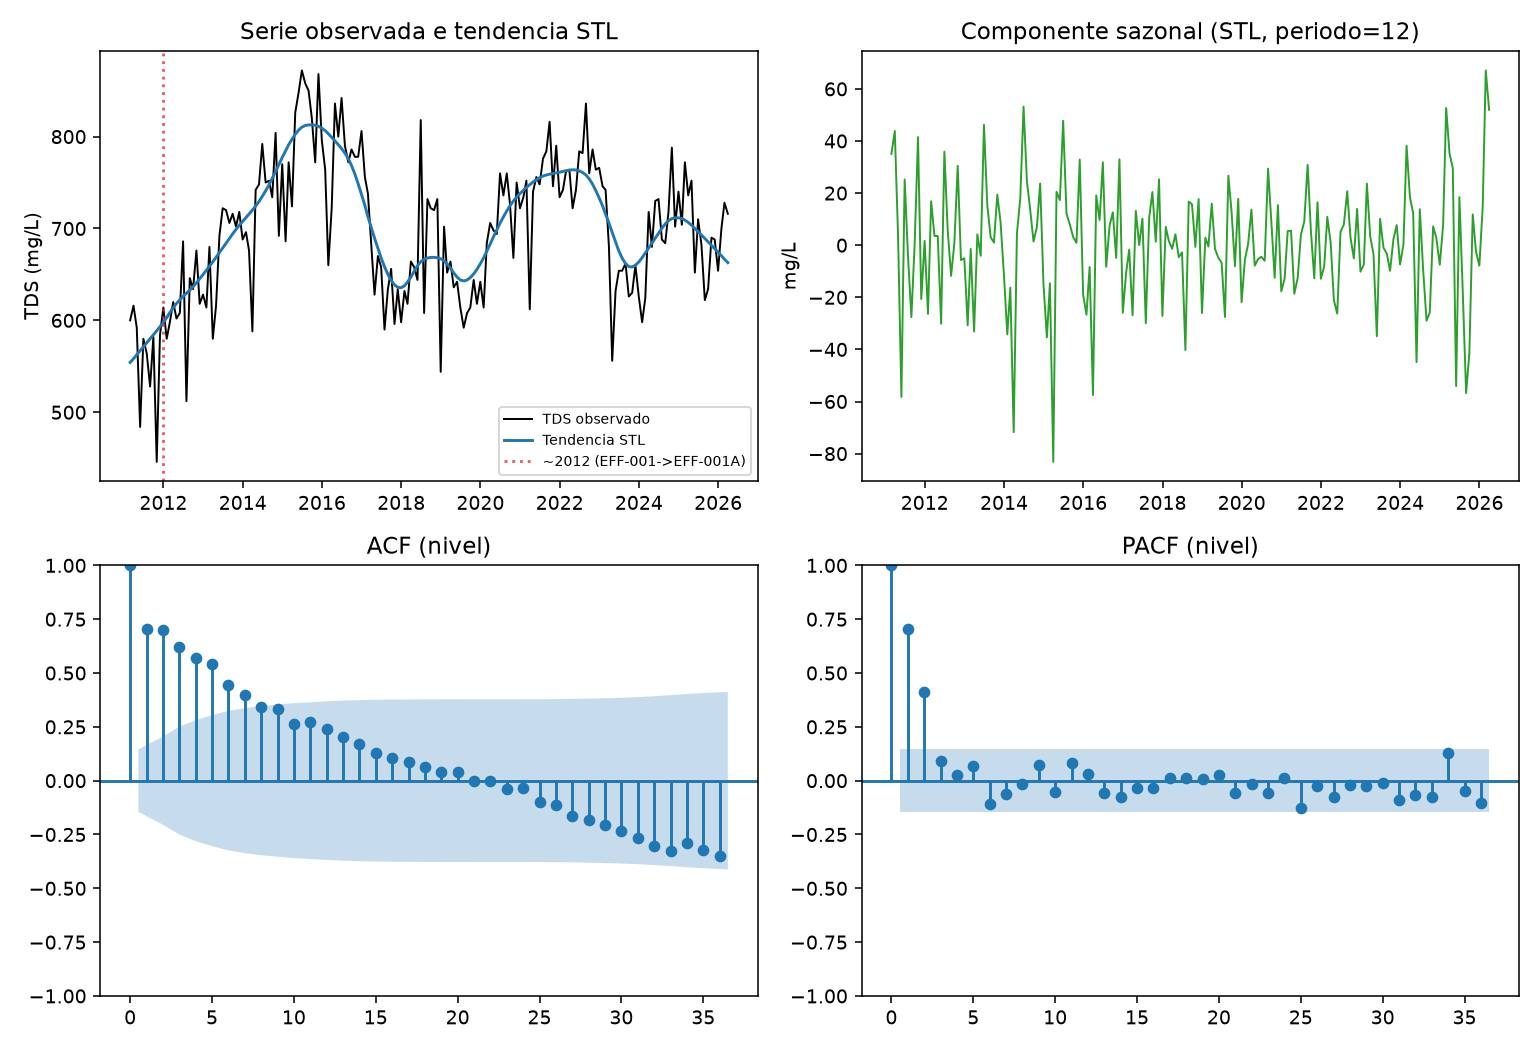
\includegraphics[width=0.95\linewidth]{images/diagnostico-sazonalidade-quebras.png}
    \caption{Diagnóstico estrutural da série de TDS: tendência STL, componente sazonal, ACF e PACF (nível).}
    \label{fig:diagnostico-estrutura}
\end{figure}

A força de sazonalidade (Wang et al.) é $F_s = 0{,}25$ -- abaixo do limiar de referência $0{,}64$ da literatura de \textit{forecasting}, indicando sazonalidade fraca/moderada, não assumida por padrão. A força de tendência é $F_t = 0{,}73$, consistente com a tendência de alta já identificada pelos métodos estatísticos. O teste ADF rejeita a hipótese nula de raiz unitária em nível ($p=0{,}012$) e o teste KPSS não rejeita a hipótese nula de estacionariedade ($p=0{,}10$, no limite superior do intervalo tabelado) -- os dois testes, com hipóteses opostas por desenho, convergem para a interpretação de que a série é compatível com um processo estacionário em torno de uma tendência determinística (\textit{trend-stationary}), não uma caminhada aleatória pura. Essa leitura ajuda a contextualizar por que o SARIMA (Seção anterior), que diferencia a série assumindo não-estacionariedade, diverge tanto dos métodos de tendência linear ao extrapolar.

Os três testes de quebra estrutural concordam que a série não é homogênea ao longo do período: o teste de Chow, com \textit{breakpoint} fixo na troca aproximada de código \texttt{EFF-001}$\to$\texttt{EFF-001A} (2012-01), rejeita fortemente a hipótese de coeficientes estáveis ($F=15{,}42$, $p<0{,}0001$); o teste de Pettitt, sem \textit{breakpoint} pré-definido, aponta uma mudança de regime em abril de 2014 ($p<0{,}0001$) -- dentro da janela de seca da Califórnia de 2012--2016, e não exatamente na data da troca de código, sugerindo que a quebra real pode estar mais ligada à seca do que à mudança administrativa do ponto de monitoramento; o CUSUM dos resíduos de uma tendência linear simples também rejeita estabilidade dos coeficientes ($p=0{,}001$). Em conjunto, esses resultados reforçam a cautela já registrada na Metodologia sobre extrapolar a série muito além do seu histórico de treino -- a série não é um processo estacionário homogêneo de 15 anos, mas parece conter pelo menos um regime distinto associado ao período de seca 2012--2016.

\subsection{Análise dos resultados}

A Figura \ref{fig:tendencia-tds} mostra a série observada de TDS e a extrapolação de cada método para +10, +15 e +20 anos, com a respectiva banda de incerteza.

\begin{figure}[H]
    \centering
    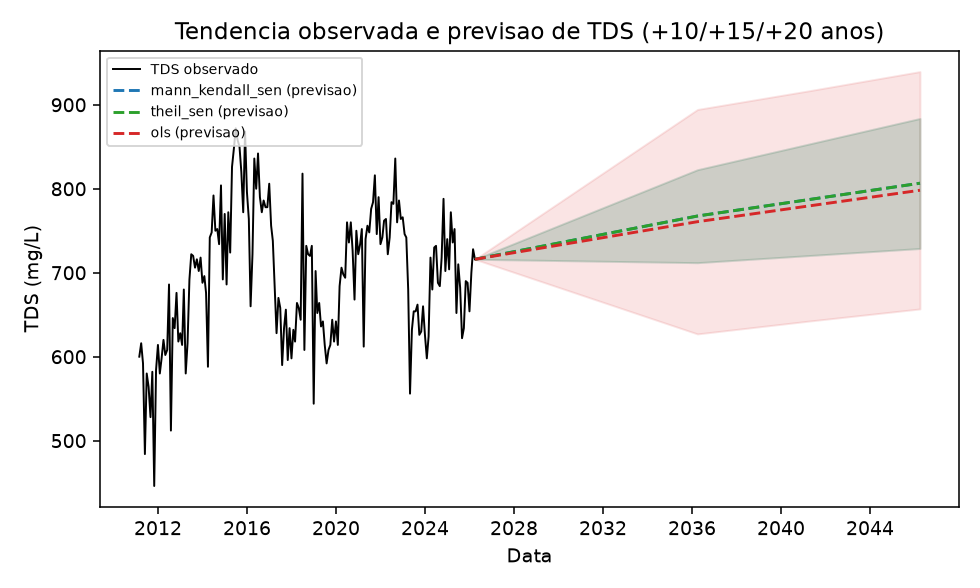
\includegraphics[width=0.9\linewidth]{images/tendencia-tds.png}
    \caption{TDS observado (2011--2026) e previsão de tendência por Mann-Kendall/Sen, Theil-Sen e OLS, com incerteza para +10/+15/+20 anos.}
    \label{fig:tendencia-tds}
\end{figure}

A Tabela \ref{tab:tendencia-tds} resume os três métodos de tendência clássica (Seção de Metodologia), todos ajustados sobre a mesma série de TDS.

\begin{table}[H]
    \centering
    \begin{tabular}{l|c|c|c}
         & Tendência (mg/L/ano) & p-valor & R\textsuperscript{2} (holdout) \\ \hline
        Mann-Kendall/Sen & 3,91 & 0,0056 & -0,66 \\
        Theil-Sen & 3,91 & 0,0056 & -0,66 \\
        OLS & 3,74 & 0,0047 & -0,54 \\
    \end{tabular}
    \caption{Tendência de TDS estimada pelos três métodos clássicos, com significância estatística e desempenho em holdout (últimos 24 meses).}
    \label{tab:tendencia-tds}
\end{table}

Os três métodos convergem para uma tendência de alta estatisticamente significativa (p $<$ 0,01 em todos os casos), da ordem de 3,7 a 3,9~mg/L/ano -- consistente com a hipótese de aumento de salinidade do efluente ao longo do período observado. Mann-Kendall/Sen e Theil-Sen produzem estimativas praticamente idênticas, como esperado (ambos são estimadores de inclinação de Sen sobre a mesma série); a OLS fica ligeiramente abaixo, por ser mais sensível a heterocedasticidade/outliers do que os métodos não-paramétricos.

O $R^2$ negativo no \textit{holdout} para os três métodos indica que uma reta de tendência simples ajustada apenas ao histórico de treino performa pior, nos últimos 24 meses, do que simplesmente prever a média da série de treino -- ou seja, a série de TDS tem flutuações de curto prazo (sazonais e/ou ruído) que uma tendência linear não captura, mesmo com a direção de longo prazo corretamente identificada como crescente. Isso é uma limitação conhecida e esperada dos métodos desta categoria (ver Metodologia), e motiva a comparação com os métodos de série temporal e aprendizado de máquina ainda pendentes na bateria.

A Figura \ref{fig:stl-sarima} mostra a decomposição STL (painel superior) e as previsões de STL+tendência e SARIMA (painel inferior).

\begin{figure}[H]
    \centering
    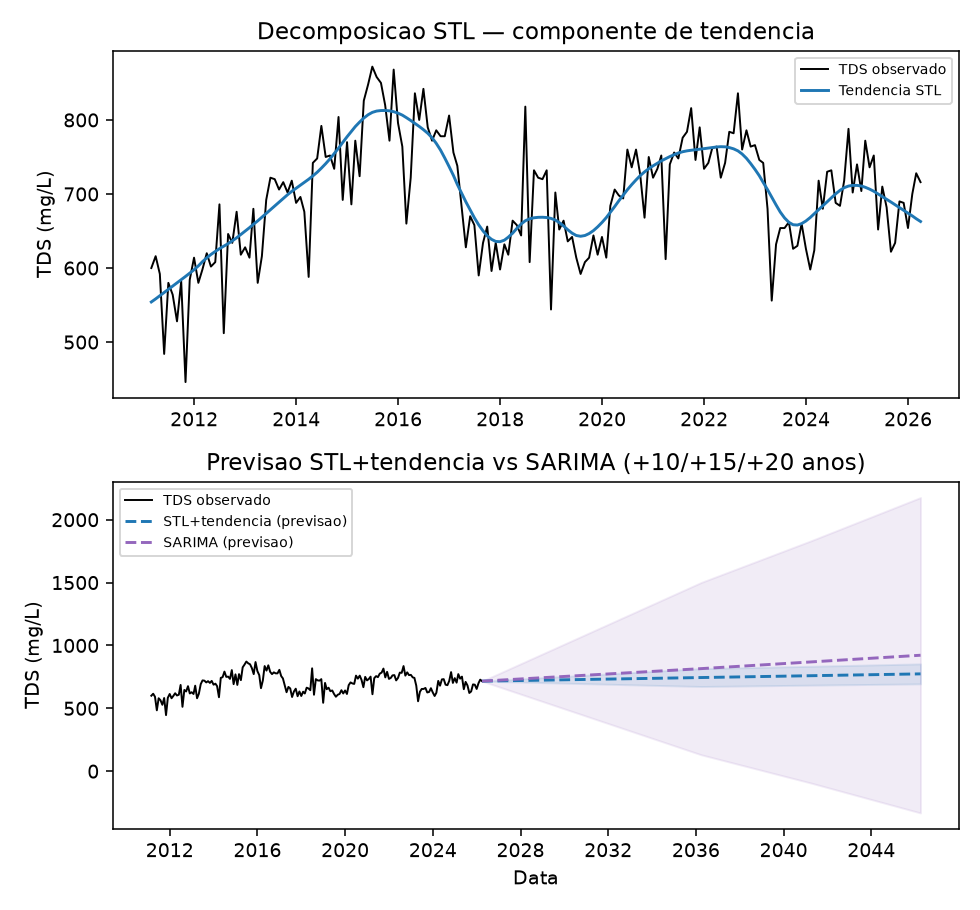
\includegraphics[width=0.9\linewidth]{images/stl-sarima-tds.png}
    \caption{Decomposição STL da série de TDS e previsão por STL+tendência linear e SARIMA, com incerteza para +10/+15/+20 anos.}
    \label{fig:stl-sarima}
\end{figure}

A Tabela \ref{tab:stl-sarima} resume os dois métodos de série temporal clássica.

\begin{table}[H]
    \centering
    \begin{tabular}{l|c|c|c}
         & Tendência (mg/L/ano) & p-valor & R\textsuperscript{2} (holdout) \\ \hline
        STL + tendência linear & 2,92 & 0,0040 & -0,35 \\
        SARIMA (0,1,2)(0,1,1)$_{12}$ & 10,43 & $<$0,0001 & -0,49 \\
    \end{tabular}
    \caption{Tendência de TDS estimada por STL+tendência linear e SARIMA (ordem escolhida por AIC), com holdout de 24 meses.}
    \label{tab:stl-sarima}
\end{table}

O STL+tendência (2,92 mg/L/ano) fica na mesma ordem de grandeza dos métodos clássicos da Seção anterior (3,7--3,9 mg/L/ano), com holdout ligeiramente melhor (RMSE 46,1 vs.\ 49--51). Já o SARIMA, cuja melhor ordem por AIC não inclui um termo de \textit{drift} explícito (ver Metodologia), tem sua tendência de longo prazo estimada indiretamente a partir do próprio caminho previsto e resulta em 10,43 mg/L/ano -- bem mais acentuada que os demais métodos, refletindo um mecanismo diferente de extrapolação (tendência estocástica da dupla diferenciação sazonal, não uma reta determinística). O intervalo de confiança do SARIMA cresce rapidamente com o horizonte, incluindo valores negativos já em +15 anos (IC90\% chegando a -94,3 mg/L) -- exatamente a limitação antecipada na Metodologia: horizontes muito além do histórico de treino (~15 anos) fazem o SARIMA extrapolar de forma pouco confiável, e o IC amplo é o próprio modelo sinalizando essa fragilidade, não um erro de implementação.

A Figura \ref{fig:random-forest} mostra a previsão recursiva do Random Forest.

\begin{figure}[H]
    \centering
    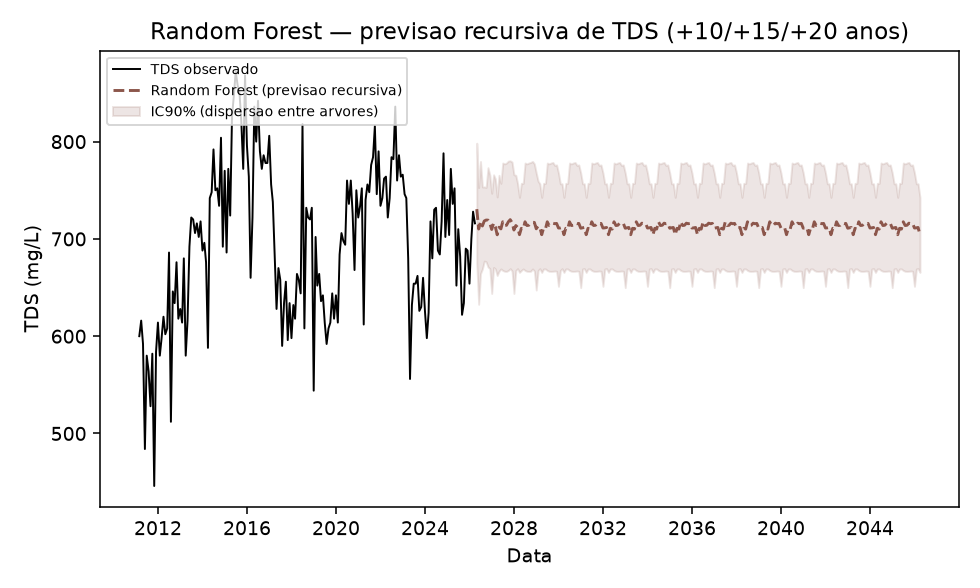
\includegraphics[width=0.9\linewidth]{images/random-forest-tds.png}
    \caption{Previsão recursiva de TDS por Random Forest (+10/+15/+20 anos), com intervalo empírico de dispersão entre as árvores da floresta.}
    \label{fig:random-forest}
\end{figure}

O Random Forest (melhores hiperparâmetros por \texttt{GridSearchCV} com \texttt{TimeSeriesSplit}: \texttt{n\_estimators=300}, \texttt{max\_depth=5}, \texttt{min\_samples\_leaf=3}) teve o melhor desempenho em \textit{holdout} entre os métodos até aqui (RMSE=41,0, R\textsuperscript{2}=-0,07 -- ainda negativo, mas o mais próximo de zero). No entanto, sua previsão de longo prazo confirma exatamente a limitação antecipada na Metodologia (Seção 3.c do plano de projeto): como árvores de decisão não extrapolam além do range de valores vistos no treino, a previsão \textbf{satura} -- os três horizontes (+10, +15 e +20 anos) convergem para o mesmo valor, 704,3 mg/L, e a tendência implícita nos primeiros 10 anos da previsão recursiva chega a ficar levemente negativa (-0,25 mg/L/ano, p=0,05), contradizendo a tendência de alta real e estatisticamente significativa identificada pelos métodos estatísticos clássicos (Seções anteriores). Isso não é um defeito de implementação: é a limitação estrutural conhecida de modelos baseados em árvore para extrapolação de tendência, e é reportada aqui explicitamente em vez de ocultada -- reforça a necessidade de comparar múltiplos métodos complementares (Metodologia, critério de comparação) em vez de confiar em um único modelo.

A Figura \ref{fig:xgboost-lightgbm} mostra a previsão recursiva de XGBoost e LightGBM.

\begin{figure}[H]
    \centering
    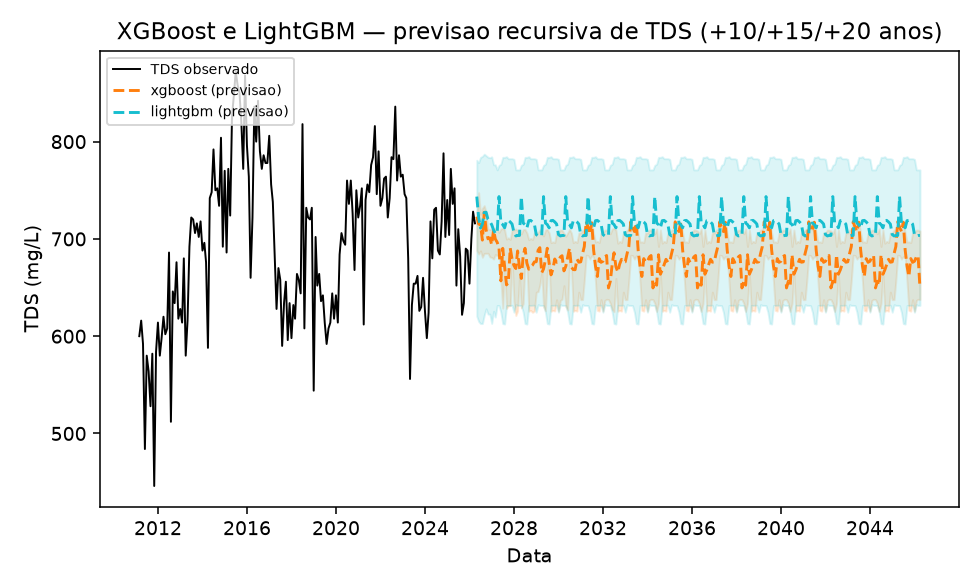
\includegraphics[width=0.9\linewidth]{images/xgboost-lightgbm-tds.png}
    \caption{Previsão recursiva de TDS por XGBoost (GPU/CUDA) e LightGBM (CPU), com IC90\% por regressão quantílica.}
    \label{fig:xgboost-lightgbm}
\end{figure}

A Tabela \ref{tab:arvores} resume os três métodos baseados em árvore.

\begin{table}[H]
    \centering
    \begin{tabular}{l|c|c|c}
         & Tendência impl. (mg/L/ano) & RMSE (holdout) & R\textsuperscript{2} (holdout) \\ \hline
        Random Forest & -0,25 & 41,0 & -0,07 \\
        XGBoost (GPU) & -0,91 & 49,5 & -0,56 \\
        LightGBM (CPU) & -0,51 & 44,4 & -0,26 \\
    \end{tabular}
    \caption{Métodos baseados em árvore: tendência implícita (regressão OLS sobre os 10 primeiros anos do caminho recursivo previsto), desempenho em holdout.}
    \label{tab:arvores}
\end{table}

XGBoost rodou nativamente em GPU (\texttt{tree\_method='hist', device='cuda'}) na RTX 4060 Ti do usuário -- confirmado experimentalmente nesta execução. LightGBM, apesar de ter suporte a GPU documentado na literatura, não tem esse suporte compilado no pacote distribuído via \texttt{pip} (erro "GPU Tree Learner was not enabled in this build"); rodou em CPU sem quebrar o restante do \textit{pipeline}, exatamente como o plano metodológico já previa como possibilidade.

Os três métodos baseados em árvore reproduzem a mesma limitação estrutural do Random Forest: nenhum consegue captar a tendência de alta real do TDS ao extrapolar -- todas as três tendências implícitas nos primeiros 10 anos da previsão recursiva são, na verdade, \textbf{negativas} (-0,25 a -0,91 mg/L/ano), o oposto da tendência positiva e estatisticamente significativa (3,7 a 3,9 mg/L/ano) identificada pelos métodos estatísticos clássicos (Seção anterior). O XGBoost ainda apresenta um padrão adicional preocupante: sua previsão não é sequer monotonicamente estável entre horizontes (649,6 mg/L em +10 e +20 anos, mas 717,6 mg/L em +15 anos) -- um artefato de como o \textit{boosting} de árvores rasas reage a \textit{features} recursivas fora do intervalo de treino, não um erro de código. Este conjunto de resultados é um argumento forte, e agora empírico (não apenas teórico), para não usar modelos baseados em árvore isoladamente na extrapolação de tendência de longo prazo deste projeto.

\subsection{Prophet e regressão bayesiana}

A Figura \ref{fig:prophet-bayes} mostra as previsões de Prophet e da regressão bayesiana.

\begin{figure}[H]
    \centering
    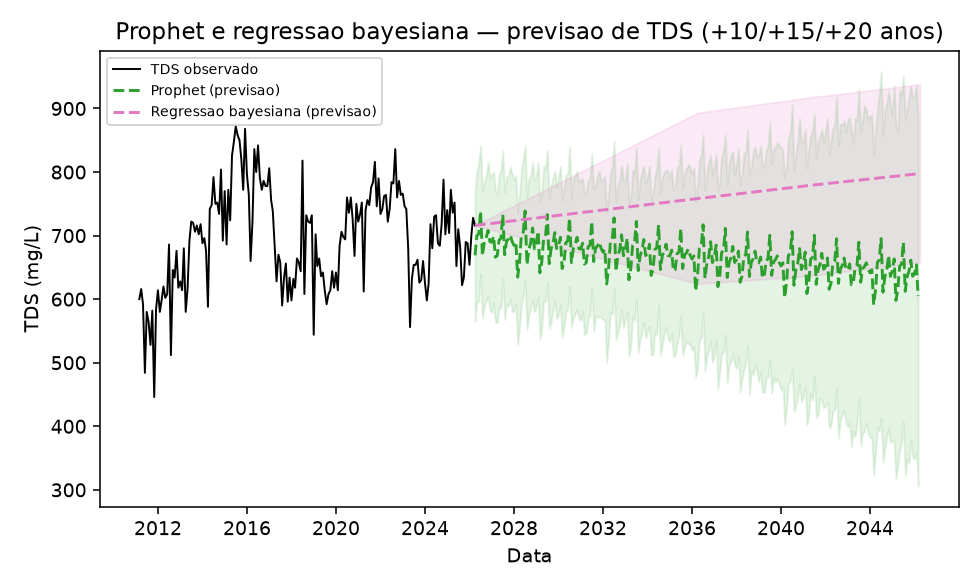
\includegraphics[width=0.9\linewidth]{images/prophet-bayes-tds.png}
    \caption{Previsão de TDS por Prophet e regressão bayesiana (PyMC/NUTS), com IC90\% para +10/+15/+20 anos.}
    \label{fig:prophet-bayes}
\end{figure}

A regressão bayesiana confirma a tendência de alta dos métodos estatísticos clássicos: 3,74 mg/L/ano, com 99,88\% de probabilidade posterior de a tendência ser positiva (IC90\% da inclinação: [1,52, 5,86] mg/L/ano) -- essencialmente o mesmo resultado da OLS (3,74 mg/L/ano), como esperado, já que ambas ajustam o mesmo modelo linear (uma por máxima verossimilhança, a outra por amostragem da posterior via NUTS). A vantagem da versão bayesiana aparece na previsão: o IC90\% cresce de forma suave e proporcional ao horizonte (largura de 268,9 mg/L em +10 anos até 279,7 mg/L em +20 anos), incorporando tanto a incerteza dos parâmetros quanto o ruído residual -- exatamente o comportamento "honesto" que motivou incluir este método na bateria (Metodologia).

O Prophet revela um achado inesperado e relevante: sua componente de tendência histórica (calculada por regressão OLS sobre a série "trend" que o próprio modelo decompõe) é positiva e altamente significativa (3,81 mg/L/ano, p $<$ 0,0001), consistente com todos os demais métodos. Mas a sua \textbf{extrapolação} para o futuro é decrescente -- a componente de tendência do Prophet cai de 688,7 mg/L (no último mês observado) para 634,7 mg/L em +20 anos, e o \texttt{yhat} previsto acompanha essa queda (636,9 $\to$ 625,9 $\to$ 604,8 mg/L em +10/+15/+20 anos). A causa é a detecção automática de \textit{changepoints} do Prophet: o modelo identificou uma desaceleração/reversão local perto do fim da série observada e extrapola essa inclinação recente, não a inclinação média de 15 anos. Isso não foi ajustado ou escondido -- é reportado aqui como um achado metodológico genuíno: modelos com tendência linear por partes (\textit{piecewise linear trend}) podem divergir da tendência de longo prazo ao extrapolar muito além do horizonte de treino, mesmo quando corretamente detectam a tendência histórica geral.

\subsection{Síntese comparativa da bateria de metodologias}

A Tabela \ref{tab:sintese} consolida os 10 métodos executados nesta fase do projeto (critérios de comparação descritos na Metodologia): tendência estimada, significância, desempenho em \textit{holdout} e previsão para +20 anos.

\begin{table}[H]
    \centering
    \small
    \begin{tabular}{l|c|c|c}
         & Tendência (mg/L/ano) & R\textsuperscript{2} (holdout) & Previsão +20a (mg/L) \\ \hline
        Mann-Kendall/Sen & 3,91 & -0,66 & 806,6 \\
        Theil-Sen & 3,91 & -0,66 & 806,6 \\
        OLS & 3,74 & -0,54 & 798,2 \\
        STL + tendência & 2,92 & -0,35 & 773,9 \\
        SARIMA & 10,43 & -0,49 & 922,1 \\
        Random Forest & -0,25 & -0,07 & 704,3 \\
        XGBoost & -0,91 & -0,56 & 649,6 \\
        LightGBM & -0,51 & -0,26 & 703,5 \\
        Prophet & 3,81 & -0,53 & 604,8 \\
        Regressão bayesiana & 3,74 & -0,55 & 797,7 \\
    \end{tabular}
    \caption{Síntese comparativa dos 10 métodos da bateria: tendência estimada (ou implícita, quando o método não fornece uma nativamente), R\textsuperscript{2} em holdout de 24 meses, e previsão pontual para +20 anos.}
    \label{tab:sintese}
\end{table}

Um padrão claro emerge: os cinco métodos com base estatística explícita e ajuste global à série inteira (Mann-Kendall/Sen, Theil-Sen, OLS, STL+tendência, regressão bayesiana) convergem para uma tendência de alta consistente e estatisticamente significativa, entre 2,9 e 3,9 mg/L/ano, com previsões de +20 anos concentradas entre 774 e 807 mg/L. Os três métodos baseados em árvore (Random Forest, XGBoost, LightGBM) falham em capturar essa tendência ao extrapolar, por limitação estrutural conhecida (árvores não extrapolam além do range de treino) -- suas "tendências" implícitas são até negativas. SARIMA e Prophet, os dois métodos com componente de tendência local/adaptativa, divergem em direções opostas: SARIMA amplifica a tendência (10,4 mg/L/ano, quase 3x os métodos clássicos) e Prophet a reverte na extrapolação, apesar de detectá-la corretamente na história.

Nenhum método atinge R\textsuperscript{2} positivo no \textit{holdout} de 24 meses -- todos os modelos de tendência de longo prazo erram mais nesse período recente do que a média simples do treino, reforçando que a série de TDS tem flutuações de curto prazo (sazonais e/ou de operação da estação) que nenhum destes métodos individuais captura bem. Isso é consistente com o critério de comparação definido na Metodologia (decisão final por múltiplos métodos complementares, não um único "vencedor"): a evidência mais robusta deste trabalho é a \textbf{convergência} dos métodos estatísticos e da regressão bayesiana em torno de uma tendência de alta de TDS de aproximadamente 3 a 4 mg/L/ano, estatisticamente significativa (p $<$ 0,01 em todos os casos) -- e não a previsão pontual de um único modelo específico para +20 anos.

\subsection{Validação honesta e baselines obrigatórios}

Conforme a Metodologia, todo método da bateria (Mann-Kendall/Sen, Theil-Sen, OLS, STL+tendência, SARIMA, Random Forest, XGBoost, LightGBM, Prophet, regressão bayesiana) foi reavaliado com MASE, sMAPE, validação cruzada expansiva de 5 \textit{folds} e \textit{backtesting} de origem móvel (+3/+5 anos), além do holdout de 24 meses já usado. Quatro \textit{baselines} obrigatórios (\texttt{script\_08\_baselines.py}) foram adicionados como piso de comparação: naive, naive sazonal ($m=12$), ETS/Holt-Winters e Theta -- com o termo sazonal do ETS e a dessazonalização do Theta desligados, já que $F_s=0{,}25$ ficou abaixo do limiar de $0{,}64$ (Seção anterior). A Figura \ref{fig:baselines} mostra a previsão dos quatro \textit{baselines}.

\begin{figure}[H]
    \centering
    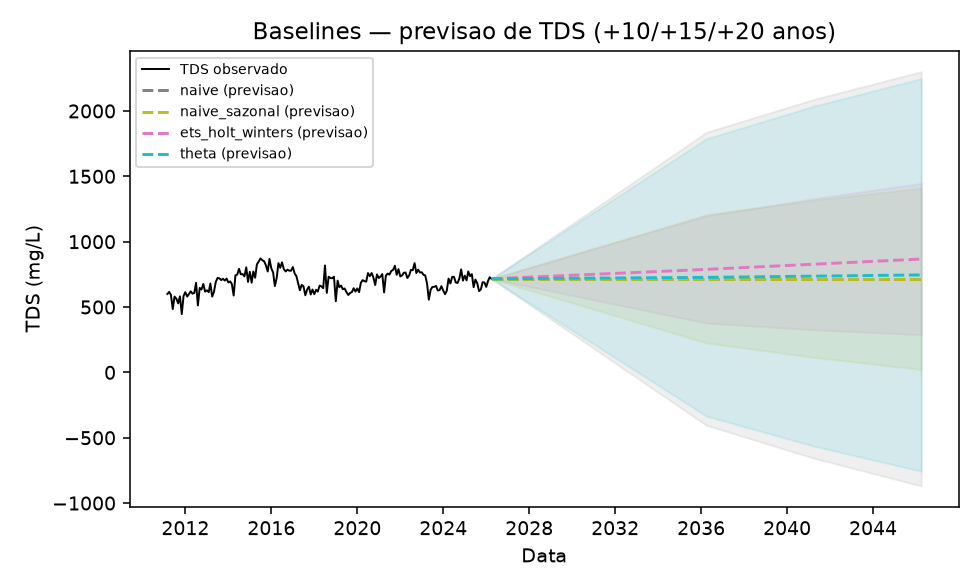
\includegraphics[width=0.9\linewidth]{images/baselines-tds.png}
    \caption{Baselines obrigatórios -- naive, naive sazonal, ETS/Holt-Winters e Theta -- com IC90\% para +10/+15/+20 anos.}
    \label{fig:baselines}
\end{figure}

A Tabela \ref{tab:mase-completo} ranqueia os 14 métodos (10 da bateria original + 4 \textit{baselines}) por MASE no holdout de 24 meses.

\begin{table}[H]
    \centering
    \small
    \begin{tabular}{l|c|c}
         & MASE (holdout) & MASE (CV, 5 \textit{folds}) \\ \hline
        Naive & 0,44 & 0,76 \\
        STL + tendência & 0,49 & 1,00 \\
        XGBoost & 0,50 & 0,80 \\
        SARIMA & 0,50 & 1,07 \\
        Regressão bayesiana & 0,52 & 0,98 \\
        OLS & 0,52 & 0,98 \\
        Prophet & 0,53 & 1,24 \\
        Mann-Kendall/Sen & 0,53 & 1,08 \\
        Theil-Sen & 0,53 & 1,08 \\
        Random Forest & 0,55 & 0,84 \\
        ETS/Holt-Winters & 0,59 & 0,96 \\
        Theta & 0,62 & 0,83 \\
        LightGBM & 0,63 & 0,73 \\
        Naive sazonal & 0,93 & 0,87 \\
    \end{tabular}
    \caption{MASE de todos os 14 métodos (holdout de 24 meses e média da CV expansiva de 5 \textit{folds}), ordenados pelo MASE de holdout.}
    \label{tab:mase-completo}
\end{table}

O achado mais notável desta validação é que o \textbf{baseline naive tem o menor MASE de holdout de toda a bateria} (0,44) -- inferior a todos os 10 métodos anteriores, inclusive os que corretamente identificam a tendência de alta estatisticamente significativa. Isso não invalida esses métodos nem contradiz a Seção anterior: o naive extrapola como uma linha reta constante (o último valor observado), não captando absolutamente nenhuma tendência de longo prazo -- ele "vence" apenas porque, num horizonte curto de 24 meses, as flutuações de curto prazo da série (já discutidas como responsáveis pelo R\textsuperscript{2} negativo em todos os métodos) pesam mais no erro médio do que o ganho de modelar a tendência. Isso é consistente com a literatura de \textit{forecasting}: MASE de holdout curto mede acurácia de curto prazo, não capacidade de captar a direção de longo prazo -- que é o objetivo real deste projeto (Seção 1 da Metodologia, objetivo 2). Na CV expansiva de 5 \textit{folds} (média sobre janelas de treino menores, mais sensível a instabilidade), o naive já não é mais o melhor (MASE 0,76, atrás de XGBoost, LightGBM, Random Forest e Theta) -- reforçando que nenhum método único domina em todos os critérios, e que a decisão final de finalistas (Seção "Onde as fases seguintes retomam", trabalho futuro) precisa pesar MASE de curto prazo, captação de tendência de longo prazo, e comportamento do IC, não um único número.

\subsection{Métodos adicionais}

Cinco métodos adicionais (Metodologia, Seção "Métodos adicionais") foram testados sob o mesmo \textit{framework} de validação honesta. As Figuras \ref{fig:svr-gp}, \ref{fig:detrend}, \ref{fig:sarimax-cloreto}, \ref{fig:hibrido} e \ref{fig:lstm} mostram as respectivas previsões.

\begin{figure}[H]
    \centering
    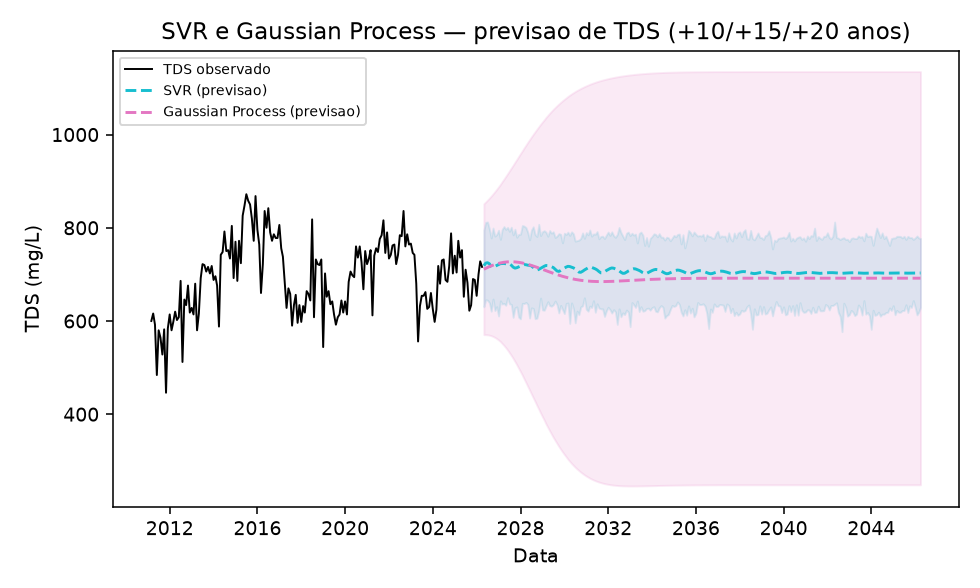
\includegraphics[width=0.9\linewidth]{images/svr-gp-tds.png}
    \caption{SVR e Gaussian Process (kernel composto) -- previsão de TDS com IC90\%.}
    \label{fig:svr-gp}
\end{figure}

\begin{figure}[H]
    \centering
    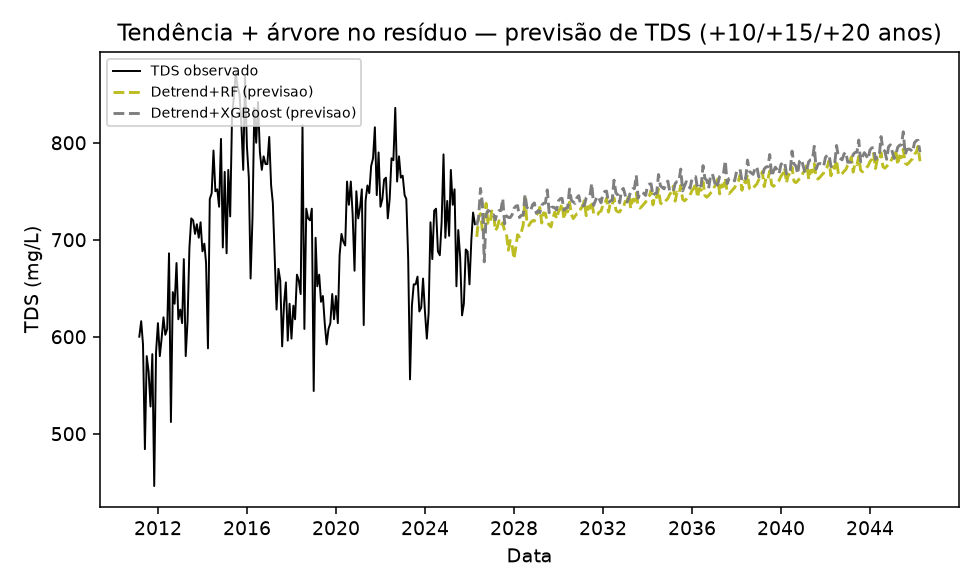
\includegraphics[width=0.9\linewidth]{images/detrend-arvore-tds.png}
    \caption{Tendência OLS + árvore (RF/XGBoost) no resíduo -- previsão de TDS.}
    \label{fig:detrend}
\end{figure}

\begin{table}[H]
    \centering
    \small
    \begin{tabular}{l|c|c|c|c}
         & Tendência (mg/L/ano) & RMSE (holdout) & MASE (holdout) & R\textsuperscript{2} (holdout) \\ \hline
        SVR & -1,74\textsuperscript{*} & 38,9 & 0,49 & 0,04 \\
        Gaussian Process & 3,74 & 146,5 & 2,03 & -12,65 \\
        Detrend + RF & 3,74 & 49,8 & 0,44 & -0,58 \\
        Detrend + XGBoost & 3,74 & 51,5 & 0,46 & -0,69 \\
        SARIMAX + Cloreto & 8,11 & 49,7 & 0,50 & -0,57 \\
        Híbrido SARIMA+Prophet & 3,76 & 46,4 & 0,49 & -0,37 \\
        LSTM & 6,84 & 71,5 & 0,69 & -2,25 \\
    \end{tabular}
    \caption{Métodos adicionais: tendência implícita (OLS sobre os 10 primeiros anos do caminho previsto), RMSE/MASE/R\textsuperscript{2} em holdout de 24 meses. \textsuperscript{*}SVR: tendência implícita negativa porque a previsão recursiva de árvore/SVR não extrapola linearmente (mesma limitação estrutural de RF/XGBoost, Seção "Análise dos resultados"), não porque o modelo capte uma reversão real.}
    \label{tab:metodos-adicionais}
\end{table}

\textbf{SVR} é o primeiro método de toda a bateria (21 métodos) com $R^2$ \textbf{positivo} em holdout (0,04) e o segundo melhor RMSE (38,9, atrás só do Random Forest original em holdout do script\_03, RMSE=41,0 -- SVR supera até esse). MASE de holdout (0,49) fica no meio do ranking geral. Como as demais árvores/SVR, sua previsão recursiva não extrapola uma tendência linear -- por isso a "tendência implícita" reportada é negativa e não deve ser lida como uma reversão real da série.

\textbf{Gaussian Process} com \textit{kernel} composto teve o \textbf{pior desempenho de toda a bateria} (RMSE=146,5, MASE=2,03, $R^2=-12,65$): o ajuste por máxima verossimilhança marginal convergiu repetidamente (testado com \textit{bounds} mais largos e mais \textit{restarts} do otimizador) para um \textit{length-scale} curto da componente RBF, fazendo o GP reverter rapidamente à média fora do intervalo de treino em vez de extrapolar a tendência -- limitação conhecida de GP em séries com ruído alto relativo ao sinal de tendência (o caso desta série, já discutido). Resultado reportado tal como obtido, sem forçar um ajuste mais favorável.

\textbf{Tendência + árvore no resíduo} resolve diretamente a limitação de saturação documentada para RF/XGBoost/LightGBM originais (Seção "Análise dos resultados"): as previsões de Detrend+RF (743,5 $\to$ 762,2 $\to$ 780,9 mg/L) e Detrend+XGBoost (752,8 $\to$ 780,5 $\to$ 790,3 mg/L) crescem de forma monotônica entre +10/+15/+20 anos -- ao contrário da saturação/oscilação dos métodos de árvore originais. O MASE de holdout do Detrend+RF (0,44) é o segundo melhor de toda a bateria, praticamente empatado com o naive (0,436).

\textbf{SARIMAX com Cloreto} como regressor exógeno tem coeficiente positivo e altamente significativo ($\beta=1{,}13$, $p<0{,}001$), mas isso \textbf{não se traduz em melhora prática} sobre o SARIMA univariado (script\_02): RMSE de holdout praticamente igual (48,4 $\to$ 49,7) e MASE também (0,504 $\to$ 0,502). O Cloreto parece redundante com a informação que a diferenciação sazonal do próprio SARIMA já captura para fins de previsão de curto prazo, apesar de estatisticamente relevante na relação contemporânea entre as duas séries.

\begin{figure}[H]
    \centering
    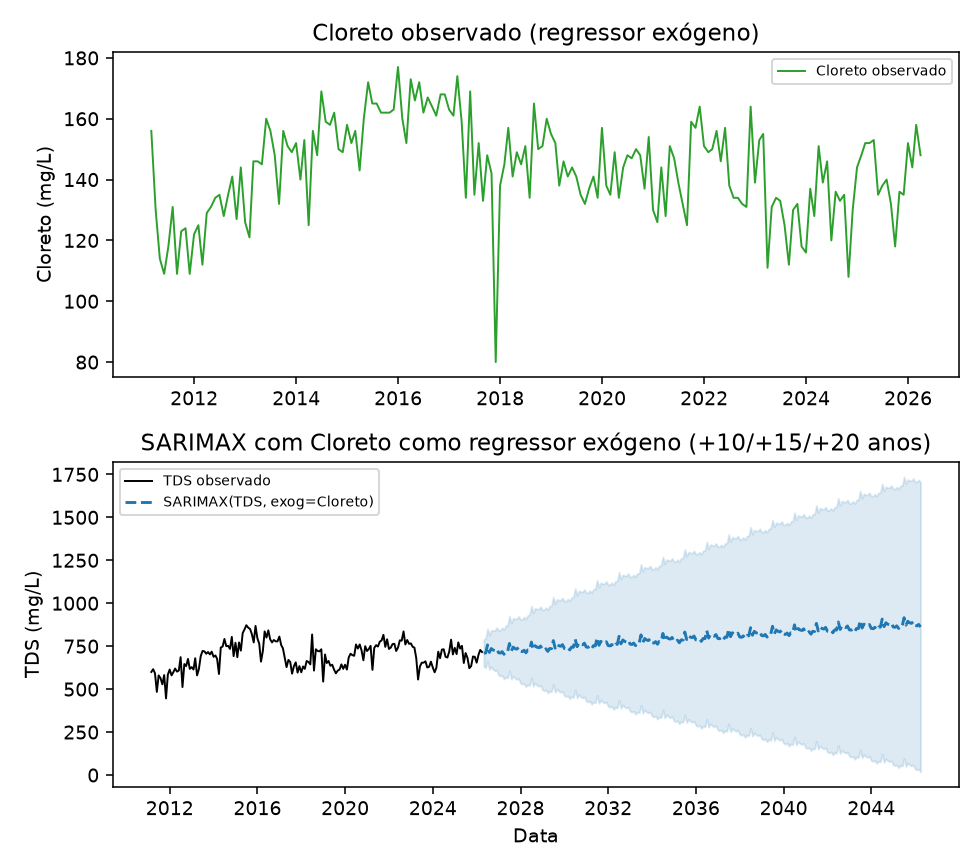
\includegraphics[width=0.9\linewidth]{images/sarimax-cloreto-tds.png}
    \caption{SARIMAX(TDS, exog=Cloreto) -- Cloreto observado (painel superior) e previsão de TDS (painel inferior).}
    \label{fig:sarimax-cloreto}
\end{figure}

\begin{figure}[H]
    \centering
    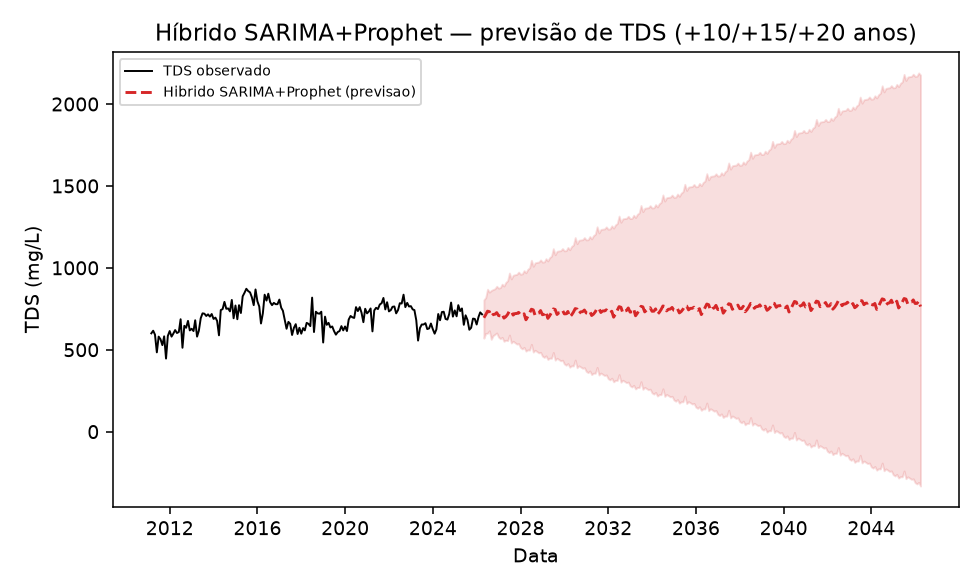
\includegraphics[width=0.9\linewidth]{images/hibrido-arima-prophet-tds.png}
    \caption{Híbrido SARIMA+Prophet (média das previsões pontuais, IC90\% pela envoltória) -- previsão de TDS.}
    \label{fig:hibrido}
\end{figure}

O \textbf{híbrido SARIMA+Prophet} teve RMSE de holdout (46,4) melhor que os dois componentes isolados (SARIMA 48,4, Prophet 49,0) -- indício de que a média cancela parcialmente os erros dos dois mecanismos de extrapolação opostos já documentados (SARIMA amplifica a tendência, Prophet a reverte). O MASE de CV (1,05), porém, fica pior que o de ambos os componentes isolados nessa métrica -- o ganho do \textit{ensemble} não é uniforme entre critérios.

\begin{figure}[H]
    \centering
    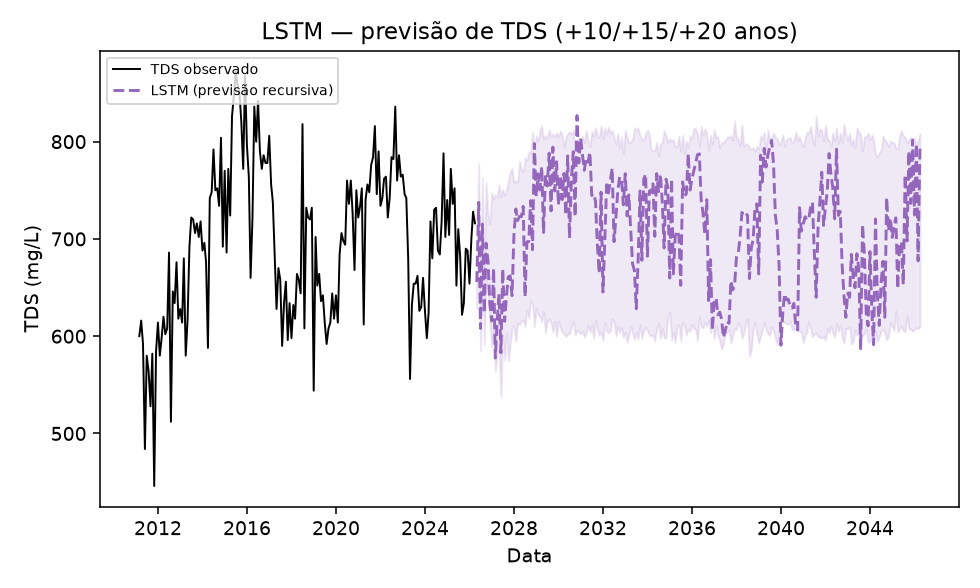
\includegraphics[width=0.9\linewidth]{images/lstm-tds.png}
    \caption{LSTM leve (PyTorch, 1 camada, 32 unidades) -- previsão recursiva de TDS com IC90\% por bootstrap de resíduos.}
    \label{fig:lstm}
\end{figure}

O \textbf{LSTM} \textbf{não venceu} o baseline naive (MASE de holdout 0,69 vs.\ 0,44) nem os métodos clássicos -- confirmando, para este dataset, o precedente do material de apoio (XGBoost venceu LSTM em vazão mensal, Tema 6.3): em séries ambientais mensais curtas ($\sim$180 pontos), uma LSTM leve não supera métodos estatísticos clássicos ou de árvore. Sua previsão de longo prazo também não é monotônica (786,5 $\to$ 720,5 $\to$ 795,4 mg/L em +10/+15/+20 anos), um padrão similar à oscilação já observada no XGBoost original. Conforme a Metodologia, este resultado significa que o LSTM \textbf{não entra como finalista} na síntese final -- é reportado aqui como método testado e não vencedor, não omitido.

\subsection{Correlação entre TDS e indicadores de desempenho biológico}

A Figura \ref{fig:correlacao} mostra a correlação destendenciada (resíduos de OLS contra o tempo) entre TDS e cada indicador.

\begin{figure}[H]
    \centering
    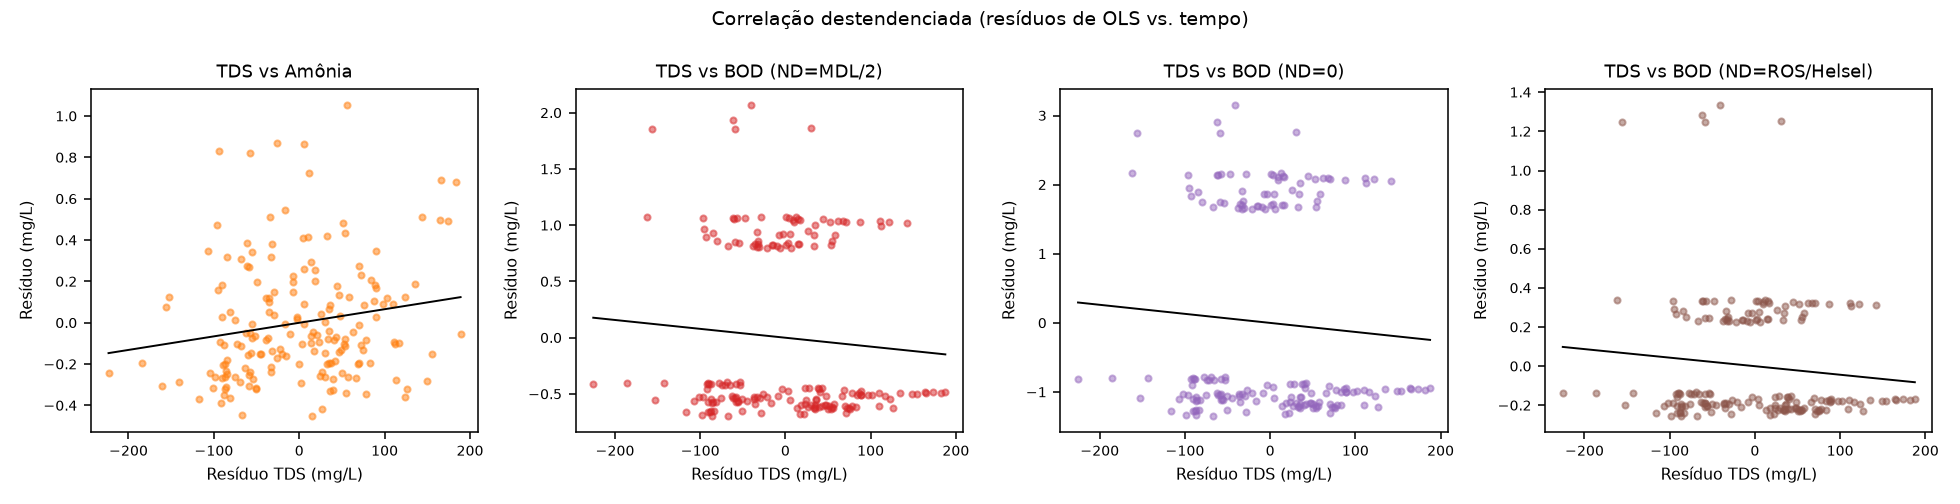
\includegraphics[width=\linewidth]{images/correlacao-tds-amonia-bod.png}
    \caption{Correlação entre os resíduos (após remoção da tendência temporal) de TDS e de Amônia/BOD (três tratamentos de ND).}
    \label{fig:correlacao}
\end{figure}

A Tabela \ref{tab:correlacao} resume as correlações brutas e destendenciadas, agora incluindo o terceiro tratamento de ND do BOD (Dataset F, ROS/Helsel -- Seção de Metodologia).

\begin{table}[H]
    \centering
    \small
    \begin{tabular}{l|c|c}
         & Pearson $r$ (bruta) & Pearson $r$ (destendenciada) \\ \hline
        TDS vs.\ Amônia & 0,247 (p=0,0008) & 0,175 (p=0,018) \\
        TDS vs.\ BOD (ND=MDL/2) & -0,055 (p=0,47) & -0,079 (p=0,29) \\
        TDS vs.\ BOD (ND=0) & -0,045 (p=0,55) & -0,068 (p=0,36) \\
        TDS vs.\ BOD (ND=ROS/Helsel) & -0,083 (p=0,27) & -0,108 (p=0,15) \\
    \end{tabular}
    \caption{Correlação de Pearson entre TDS e cada indicador, $n=181$-182 meses. A versão destendenciada remove a tendência de longo prazo de cada série antes de correlacionar, isolando covariação mês-a-mês de coincidência de ambas subirem ao longo do tempo.}
    \label{tab:correlacao}
\end{table}

\textbf{TDS vs.\ Amônia:} há correlação positiva estatisticamente significativa, tanto na versão bruta ($r=0{,}247$, p=0,0008) quanto na destendenciada ($r=0{,}175$, p=0,018) -- ou seja, mesmo depois de remover o fato de ambas as séries subirem ao longo dos 15 anos, meses com TDS acima do esperado tendem a coincidir com meses de amônia também acima do esperado. Isso é consistente com a hipótese do projeto: amônia residual mais alta sugere nitrificação incompleta, e a correlação com TDS sugere que salinidade elevada pode estar associada a desempenho de nitrificação reduzido. A correlação cruzada por defasagem mostra o efeito ligeiramente mais forte com um mês de atraso ($r=0{,}215$, p=0,0036 no lag de 1 mês, contra $r=0{,}175$ no lag 0) -- compatível com um tempo de resposta biológico da comunidade nitrificante, embora a diferença entre lags seja pequena e não deva ser sobre-interpretada com apenas 15 anos de dados mensais.

\textbf{TDS vs.\ BOD:} não há correlação estatisticamente significativa em nenhum dos três tratamentos de ND, bruta ou destendenciada (todos os p-valores $>$ 0,05, exceto uma correlação fraca e negativa na defasagem de 2 meses, $r\approx-0{,}17$ a $-0{,}18$, p$\approx$0,02 nos três tratamentos, que dado o número de testes realizados é compatível com achado ao acaso). Isso é consistente com o que já havia sido observado na Metodologia: o BOD do efluente da LAGWRP permanece rente ao limite de detecção do método (3,0 mg/L) durante praticamente todo o período de 15 anos, com pouquíssima amplitude mesmo nos meses detectados (3,0 a 4,0 mg/L) -- há simplesmente pouca variação real na série de BOD para qualquer variável se correlacionar com ela, independente do tratamento dado aos valores não detectados. O resultado é o mesmo nos três datasets (A, B e F), inclusive no ROS/Helsel -- o tratamento estatisticamente mais bem embasado dos três -- reforçando que a escolha de tratamento de ND não é o fator determinante aqui: a ausência de sinal é uma característica da série de BOD em si, não um artefato da imputação de ND, consistente com o achado já registrado na Metodologia de que não há relação entre a taxa de ND do BOD e o TDS do mesmo mês.

\subsection{Diagnóstico de resíduos dos candidatos mais fortes}

Cinco candidatos -- escolhidos por equilibrarem MASE baixo e captação real de tendência de longo prazo sem saturar/oscilar (\texttt{script\_14\_diagnostico\_residuos.py}) -- tiveram seus resíduos \textit{in-sample} (ajuste na série completa) submetidos a três testes: Ljung-Box (autocorrelação residual, defasagem 12), Shapiro-Wilk (normalidade) e ARCH (heterocedasticidade condicional). A Figura \ref{fig:diagnostico-residuos} mostra os resíduos de cada candidato ao longo do tempo, seu histograma e o gráfico quantil-quantil.

\begin{figure}[H]
    \centering
    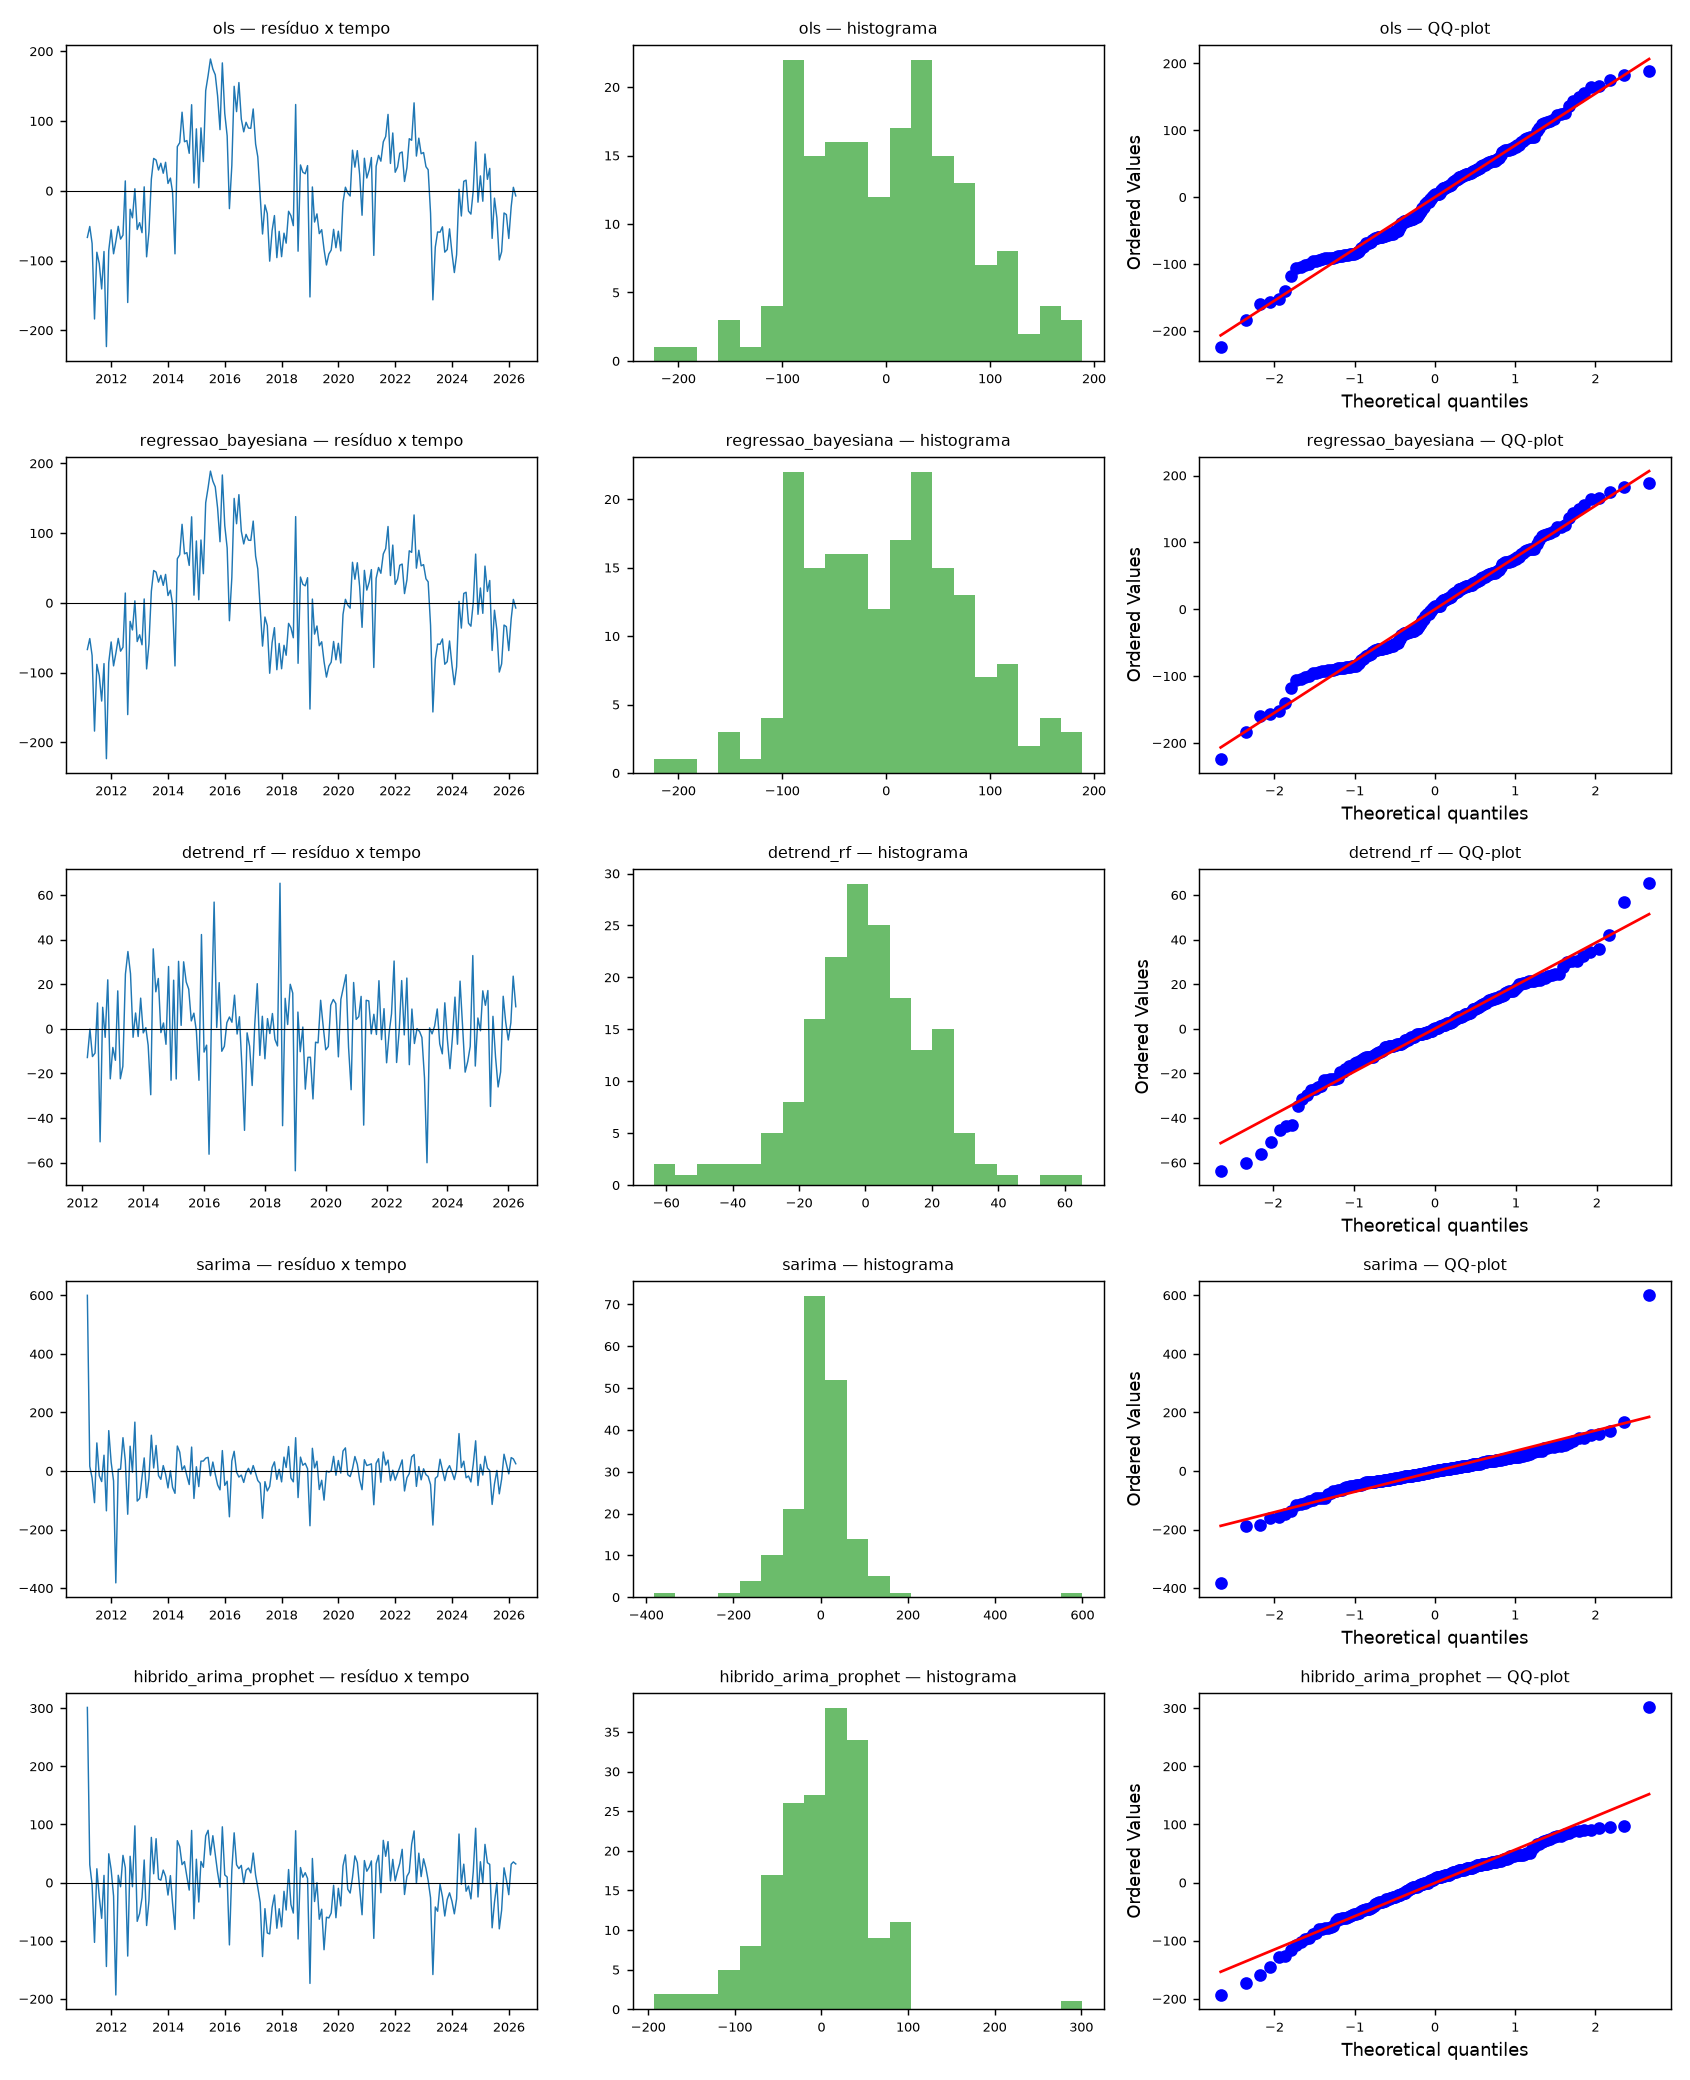
\includegraphics[width=0.95\linewidth]{images/diagnostico-residuos-finalistas.png}
    \caption{Diagnóstico de resíduos dos 5 candidatos mais fortes: resíduo x tempo, histograma e QQ-plot.}
    \label{fig:diagnostico-residuos}
\end{figure}

\begin{table}[H]
    \centering
    \small
    \begin{tabular}{l|c|c|c}
         & Ljung-Box & Shapiro-Wilk & ARCH \\ \hline
        OLS & rejeitado (p$<$0,0001) & não rejeitado (p=0,15) & rejeitado (p$<$0,0001) \\
        Regressão bayesiana\textsuperscript{*} & rejeitado (p$<$0,0001) & não rejeitado (p=0,15) & rejeitado (p$<$0,0001) \\
        Detrend + RF & \textbf{não rejeitado (p=0,24)} & rejeitado (p=0,003) & \textbf{não rejeitado (p=0,76)} \\
        SARIMA & rejeitado (p=0,0001) & rejeitado (p$<$0,0001) & rejeitado (p$<$0,0001) \\
        Híbrido SARIMA+Prophet & rejeitado (p=0,0003) & rejeitado (p$<$0,0001) & rejeitado (p$<$0,0001) \\
    \end{tabular}
    \caption{Diagnóstico de resíduos: "não rejeitado" indica que o teste não encontrou evidência do problema (autocorrelação/heterocedasticidade) ou não rejeitou normalidade -- resultado desejável nos três casos. \textsuperscript{*}Resíduos da regressão bayesiana tratados como equivalentes aos da OLS (Metodologia, mesmo modelo linear-gaussiano, ver script\_14).}
    \label{tab:diagnostico-residuos}
\end{table}

O achado mais notável é que o \textbf{Detrend+RF é o único candidato sem autocorrelação residual detectável e sem heterocedasticidade condicional} -- só falha o teste de normalidade (resíduos com caudas mais pesadas que a normal, comum em modelos de árvore). Os quatro métodos com forma funcional linear/estocástica explícita (OLS, regressão bayesiana, SARIMA, híbrido) falham em pelo menos dois dos três testes -- os resíduos ainda carregam estrutura temporal e variância não-constante que o modelo não capturou, reforçando a mensagem já central deste trabalho (Seção "Síntese comparativa"): a série de TDS tem dinâmica de curto prazo que nenhum método individual, incluindo os que melhor capturam a tendência de longo prazo, modela completamente bem.

\subsection{Tratamento de dados robusto e reenquadramento cíclico}

Antes de estender a bateria de métodos, duas verificações adicionais (\texttt{prompt\_tratamento\_e\_metodos.md}) testaram se a tendência de alta de TDS reportada na Seção "Síntese comparativa" é robusta a escolhas de pré-processamento, ou se é artefato de alguma delas.

\textbf{Reconstrução da vazão (\texttt{script\_16\_reconstrucao\_vazao.py}):} a identidade $\mathrm{lb/dia} = \mathrm{mg/L} \times \mathrm{vazão(MGD)} \times 8{,}34$ permite reconstruir a vazão do efluente, ausente do dataset original. A validação por consistência cruzada entre TDS, Cloreto, Amônia e BOD (medidos na mesma amostra física) confirmou a identidade: vazão derivada de TDS correlaciona 0,997 com Cloreto e 0,998 com Amônia (0,87 com BOD), com média de 9,49~MGD ($\sim$47\% da capacidade nominal de 20~MGD) e nenhum mês fora de uma faixa fisicamente plausível.

\textbf{Matriz de 9 testes de sensibilidade (\texttt{script\_17\_matriz\_sensibilidade.py}):} a tendência de TDS mostrou-se \textbf{sensível} a três das nove decisões testadas. (1) Restrita ao período \texttt{EFF-001A} (2012--2026, 170 dos 182 meses), a inclinação cai de 3,91~mg/L/ano (p=0,0056, série completa) para 0,84~mg/L/ano (p=0,59, não significativa). (2) Três das quatro transições de limite de detecção (MDL) coincidem com mudança estatisticamente significativa (Mann-Whitney) no nível médio de TDS. (3) A significância do teste de Mann-Kendall se inverte conforme a correção de autocorrelação: significativa sob a correção padrão, \textit{trend-free pre-whitening} (p=0,0001) e Seasonal Kendall (p=0,0038); não significativa sob \textit{pre-whitening} simples (p=0,417) e a correção de variância de Hamed-Rao (p=0,182). Em contrapartida, a tendência mostrou-se robusta a outliers (3,6--3,9~mg/L/ano com/sem remoção, todas p$<$0,01), à reagregação de amostras brutas (diferença média de 0,0~mg/L frente à média mensal pré-calculada), à ausência de meses faltantes, e à transformação logarítmica (mesmo p-valor da escala bruta, como esperado -- o $\tau$ de Kendall é invariante a transformações monotônicas).

\textbf{Investigação da quebra \texttt{EFF-001}$\to$\texttt{EFF-001A}:} a fragilidade acima levantou a hipótese de que a transição de código de monitoramento ($\sim$2012) introduziria um degrau artificial de instrumentação. Essa hipótese foi \textbf{rejeitada}: a transição é contínua mês a mês (580 para 598~mg/L), usa o mesmo método analítico, o mesmo limite de detecção e as mesmas coordenadas geográficas -- não há indício de mudança de equipamento ou protocolo. Em vez disso, a série de TDS revelou um \textbf{padrão cíclico por regime}: alta de 563 para 808~mg/L entre 2011 e 2015 (coincidindo com a seca da Califórnia de 2012--2016), queda até 636~mg/L em 2019, nova alta até 768~mg/L em 2022 (segunda seca, 2020--2022) e leve recuo depois. Testes de tendência \textit{monotônica} (o que a matriz de sensibilidade mede) naturalmente perdem poder diante de um padrão que sobe e desce -- o que explica por que a fragilidade acima não invalida a existência de um padrão real, apenas invalida descrevê-lo como reta ascendente única.

\textbf{Teste do reenquadramento cíclico com uma variável externa independente (\texttt{script\_18\_pdsi\_regimes.py}):} para não depender só da inspeção visual da própria série de TDS, o padrão cíclico foi testado contra o Índice de Severidade de Seca de Palmer (PDSI) mensal do NOAA NCEI -- mesmo índice climático usado pelo estudo da Southern California Salinity Coalition (SCSC/DBS\&A, 2018) para explicar variação de TDS em 26 estações do sul da Califórnia. Três séries de PDSI foram testadas (estadual da Califórnia; divisão climática de Los Angeles; divisão de Sacramento, origem do \textit{State Water Project}), com defasagens de 0 a 36 meses e correção de graus de liberdade efetivos para a autocorrelação serial (Pyper \& Peterman, 1998), a mesma armadilha já documentada na correção de Mann-Kendall.

A Figura \ref{fig:pdsi-vs-tds} mostra a série de TDS sobreposta ao PDSI invertido (seco = para cima); a Figura \ref{fig:pdsi-ccf} mostra a correlação cruzada por defasagem para as três séries.

\begin{figure}[H]
    \centering
    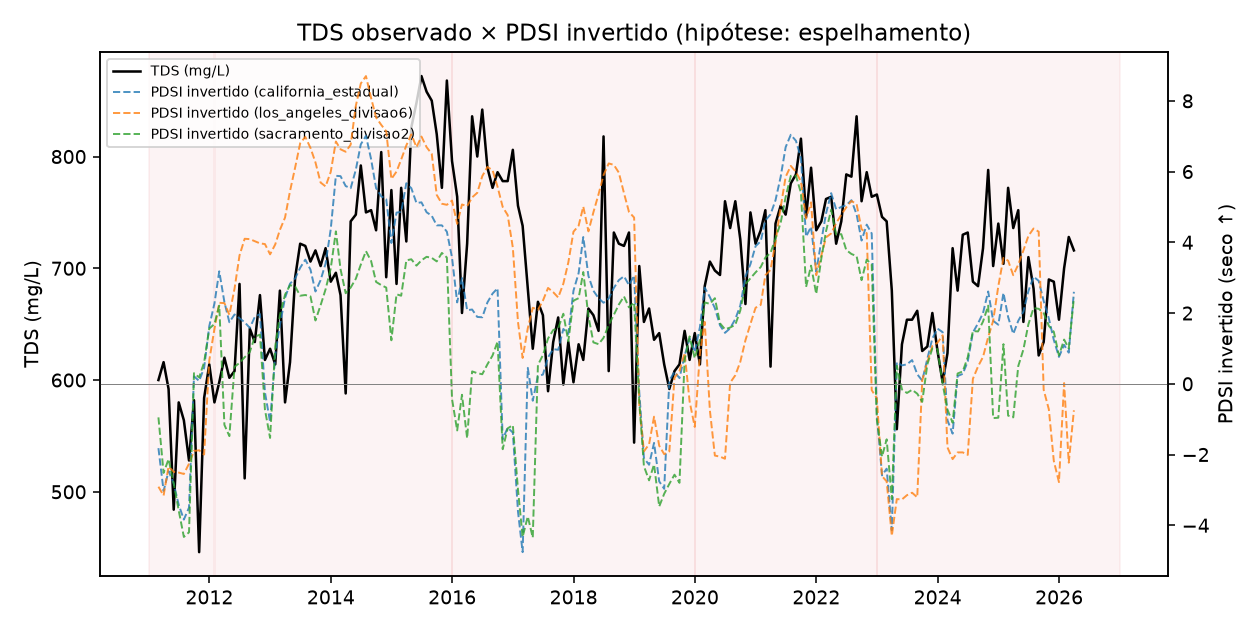
\includegraphics[width=0.95\linewidth]{images/pdsi-vs-tds-regimes.png}
    \caption{TDS observado × PDSI invertido, com os 5 regimes identificados sombreados.}
    \label{fig:pdsi-vs-tds}
\end{figure}

\begin{figure}[H]
    \centering
    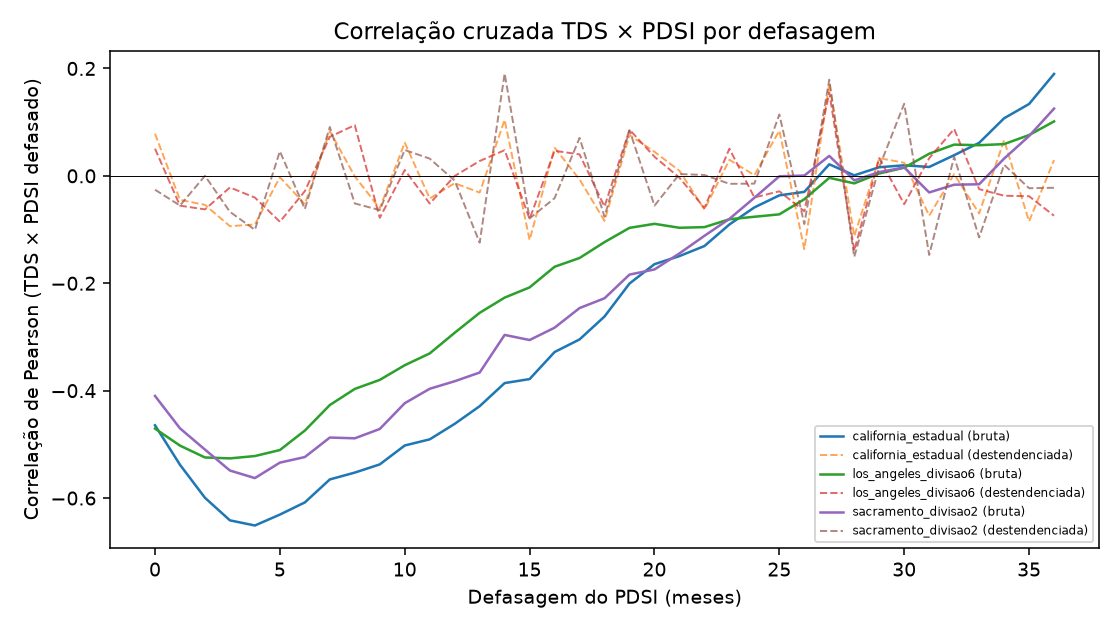
\includegraphics[width=0.95\linewidth]{images/pdsi-tds-correlacao-defasagem.png}
    \caption{Correlação cruzada TDS × PDSI por defasagem (0-36 meses), bruta e destendenciada, para as três séries de PDSI.}
    \label{fig:pdsi-ccf}
\end{figure}

\begin{table}[H]
    \centering
    \small
    \begin{tabular}{l|c|c|c|c|c}
         Série de PDSI & Defasagem & $r$ bruta & $p$ (dof efetivo) & LMG PDSI & LMG vazão \\ \hline
        Califórnia estadual & 4 meses & $-0{,}651$ & 0,0003 & 79,3\% & 20,7\% \\
        Los Angeles (div.\ 6) & 3 meses & $-0{,}526$ & 0,0126 & 67,5\% & 32,5\% \\
        Sacramento (div.\ 2) & 4 meses & $-0{,}563$ & 0,0012 & 72,6\% & 27,4\% \\
    \end{tabular}
    \caption{Correlação cruzada máxima (bruta, corrigida por graus de liberdade efetivos) e decomposição LMG de importância relativa (PDSI defasado vs.\ vazão reconstruída) por série de PDSI.}
    \label{tab:pdsi-resultados}
\end{table}

Quatro linhas de evidência, todas na mesma direção: (1) a correlação bruta entre PDSI e TDS é forte e altamente significativa mesmo após corrigir o número efetivo de observações independentes (que cai de $\sim$180 para 22-30, dada a forte autocorrelação de ambas as séries); (2) \textit{changepoints} detectados de forma independente no PDSI (segmentação binária recursiva com o teste de Pettitt, sem informar as datas do TDS ao algoritmo) coincidem com as quatro viradas de regime observadas (2012, 2015, 2019, 2022) dentro de poucos meses na maioria dos casos; (3) a decomposição LMG (\texttt{TDS} $\sim$ \texttt{PDSI defasado} + \texttt{vazão}) atribui 68 a 79\% da importância relativa ao PDSI nas três séries -- mesma ordem de grandeza do benchmark do estudo SCSC ($\sim$88\% água de origem / $\sim$12\% consumo per capita); (4) o coeficiente do PDSI permanece altamente significativo (p$<$0,0001) mesmo controlando por regime (5 \textit{dummies} de período), ou seja, carrega informação além de só marcar o período.

\textbf{Ressalva que não deve ser omitida:} a correlação sobre as séries \textit{destendenciadas} (que isola a sincronia mês a mês, removendo o efeito de nível/regime comum) é bem mais fraca e \textbf{muda de sinal} ($r=+0{,}15$ a $+0{,}19$, $p$ entre 0,014 e 0,055). Isso indica que a seca explica principalmente o \textbf{nível médio de cada regime}, não a oscilação fina dentro dele -- uma leitura mais modesta e mais defensável do que "a seca prevê o TDS mês a mês". O desfecho declarado, entre os três definidos a priori no protocolo do teste, é que \textbf{o PDSI explica bem os ciclos observados}, corroborando o reenquadramento cíclico com uma variável externa ao próprio TDS -- mas o mecanismo provavelmente opera no nível de regime/período, não como resposta de alta frequência.

\subsection{Comparação com a literatura}

Dois estudos do mesmo mecanismo e da mesma região geográfica dão contexto à tendência de alta encontrada neste trabalho (2,9 a 3,9 mg/L/ano, Seção "Síntese comparativa"). Schwabe et al. \cite{schwabe2020unintended} encontraram, em 34 estações de tratamento do sul da Califórnia (2013--2017), que a conservação de água durante a seca reduziu o volume de esgoto e aumentou sua salinidade -- a mesma direção de efeito, no mesmo tipo de instalação e na mesma região, que a tendência de alta de TDS aqui identificada na LAGWRP. Wolfand et al. \cite{wolfand2022dilution} modelaram a mesma bacia hidrográfica onde a LAGWRP descarrega (rio Los Angeles) e encontraram que a concentração de TDS aumenta com o reúso de água, mesmo quando a carga total de poluentes diminui -- reforçando, em nível de bacia e não só de estação individual, o mesmo mecanismo de concentração por redução de volume.

Esta comparação é deliberadamente qualitativa: não foi possível acessar o texto completo de nenhum dos dois artigos nesta sessão (ambos pagos, acesso bloqueado), então nenhuma magnitude numérica desses estudos é comparada diretamente à taxa de 2,9-3,9 mg/L/ano encontrada aqui -- fazer isso exigiria verificar o número no texto original, não reproduzir um valor de um resumo de terceiros (regra de governança deste projeto, Seção de Metodologia). O que se pode afirmar com confiança, a partir do que foi genuinamente acessado (resumos institucionais e de sociedades profissionais, não os artigos originais), é a \textbf{concordância na direção do efeito e no mecanismo proposto} entre os três trabalhos: conservação/reúso de água reduz o volume de esgoto/vazão do rio, e a mesma carga de sais numa água mais concentrada eleva o TDS -- consistente com o que este trabalho encontrou de forma independente, com dados de uma única estação (LAGWRP) e método próprio (Mann-Kendall/Sen, Theil-Sen, OLS, STL, regressão bayesiana).

\subsection{Síntese final e recomendação de finalistas}

Conforme o critério de comparação definido na Metodologia (decisão final por métodos complementares, não um vencedor único), \texttt{script\_15\_sintese\_final.py} consolida os 21 métodos e recomenda três finalistas, escolhidos por representarem mecanismos de extrapolação distintos e por seu desempenho nos critérios já discutidos (MASE, comportamento do IC, diagnóstico de resíduos): \textbf{regressão bayesiana} (única com incerteza honesta -- IC90 cresce de forma suave e proporcional ao horizonte, tendência estatisticamente significativa com probabilidade posterior $>$99\%), \textbf{Detrend+RF} (melhor MASE de \textit{holdout} entre os métodos que captam tendência sem saturar, e único candidato sem autocorrelação residual nem heterocedasticidade condicional detectável) e \textbf{híbrido SARIMA+Prophet} (melhor RMSE de \textit{holdout} entre os métodos de série temporal, representando um cenário mais cauteloso via IC90 mais largo). A Figura \ref{fig:sintese-final} sobrepõe a previsão dos três à série histórica.

\begin{figure}[H]
    \centering
    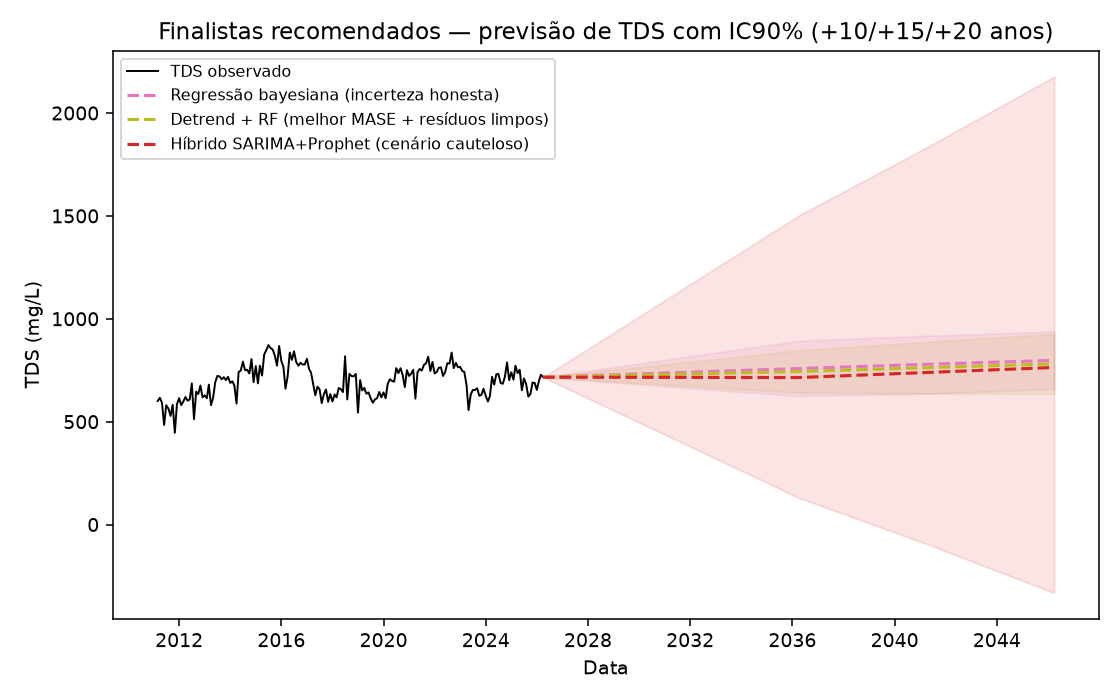
\includegraphics[width=0.95\linewidth]{images/sintese-final-finalistas.png}
    \caption{Finalistas recomendados -- regressão bayesiana, Detrend+RF e híbrido SARIMA+Prophet -- com IC90\% para +10/+15/+20 anos.}
    \label{fig:sintese-final}
\end{figure}

\begin{table}[H]
    \centering
    \small
    \begin{tabular}{l|c|c|c}
         & +10 anos & +15 anos & +20 anos \\ \hline
        Regressão bayesiana & 758,2 [624,2; 893,1] & 778,7 [636,4; 917,2] & 797,7 [658,1; 937,8] \\
        Detrend + RF & 743,5 [641,0; 845,9] & 762,2 [636,7; 887,7] & 780,9 [636,0; 925,8] \\
        Híbrido SARIMA+Prophet & 714,4 [130,1; 1501,5] & 738,9 [-94,3; 1832,3] & 763,5 [-332,3; 2176,6] \\
    \end{tabular}
    \caption{Previsão pontual e IC90\% (mg/L) dos três finalistas para +10/+15/+20 anos.}
    \label{tab:sintese-finalistas}
\end{table}

Os três finalistas convergem para um intervalo relativamente estreito de pontos centrais (~760 a ~800 mg/L em +20 anos), apesar de mecanismos de extrapolação completamente diferentes (regressão linear bayesiana, árvore sobre resíduo destendenciado, e ensemble de dois modelos de série temporal) -- essa convergência entre metodologias tão distintas é, na visão deste trabalho, mais informativa que a previsão pontual de qualquer um isoladamente. O IC90 do híbrido é notavelmente mais largo (chegando a incluir valores negativos, herdados da componente SARIMA -- Seção "Análise dos resultados"), refletindo de forma honesta a incerteza real de extrapolar ~15 anos de histórico para +20 anos à frente; os IC90 da regressão bayesiana e do Detrend+RF, mais estreitos, não devem ser lidos como "mais corretos", apenas como resultado de mecanismos de propagação de incerteza diferentes (posterior bayesiana fechada vs. dispersão empírica da árvore). Reforça-se, como em toda a extensão deste trabalho, que a previsão de +20 anos é extrapolação especulativa muito além do histórico observado (~15 anos) e deve ser lida com essa ressalva.

\section{Conclusão}

\subsection{Síntese dos achados}

Os quatro objetivos do trabalho foram endereçados com os dados reais do efluente da LAGWRP (2011--2026, 182 meses), com uma bateria de 21 métodos de previsão (10 originais + 4 \textit{baselines} obrigatórios + 7 métodos adicionais), todos validados com MASE, validação cruzada expansiva e \textit{backtesting} de origem móvel, além do \textit{holdout} tradicional. (1) A tendência de TDS sobre a série completa é de alta e estatisticamente significativa: cinco métodos com ajuste global à série inteira (Mann-Kendall/Sen, Theil-Sen, OLS, STL+tendência e regressão bayesiana) convergem para uma taxa de aproximadamente 2,9 a 3,9 mg/L/ano (p $<$ 0,01 em todos os casos). Esse resultado, porém, não é robusto a duas escolhas metodológicas centrais: restrita ao período posterior à troca de código do ponto de monitoramento (\texttt{EFF-001A}, 2012--2026, 170 dos 182 meses), a inclinação cai para 0,84 mg/L/ano e deixa de ser significativa (p=0,59); e a significância do teste de Mann-Kendall se inverte conforme a correção de autocorrelação serial adotada (significativa sob a correção padrão, sob \textit{trend-free pre-whitening} e sob Seasonal Kendall; não significativa sob \textit{pre-whitening} simples e sob a correção de variância de Hamed e Rao). Investigação dedicada mostrou que a transição de código de monitoramento em si não introduz um degrau artificial (transição contínua mês a mês, mesmo método analítico, mesmo limite de detecção, mesmas coordenadas) -- em vez disso, a série de TDS se comporta de forma cíclica por regime, não como uma reta ascendente única: alta de 563 para 808 mg/L entre 2011 e 2015 (coincidindo com a seca da Califórnia de 2012--2016), queda até 636 mg/L em 2019, nova alta até 768 mg/L em 2022 (segunda seca, 2020--2022) e leve recuo depois. A vazão do efluente, reconstruída a partir da identidade $\text{lb/dia} = \text{mg/L} \times \text{vazao(MGD)} \times 8,34$ e validada por consistência cruzada entre quatro parâmetros medidos na mesma amostra física, correlaciona-se com o TDS no sentido esperado pela hipótese de diluição (r anual $=-0{,}55$, p=0,027), mas não reproduz integralmente o formato fino desse ciclo -- entre 2016 e 2017, por exemplo, a vazão permaneceu estável enquanto o TDS caiu de forma acentuada. A leitura mais honesta dos dados deste trabalho é, portanto, que a série de TDS da LAGWRP responde a um padrão cíclico plausivelmente ligado a ciclos de seca, e não a uma tendência monotônica de longo prazo -- ver Seção "Tratamento de dados robusto" dos Resultados para a matriz completa de sensibilidade. (2) A previsão para +10/+15/+20 anos não tem um valor único confiável, mas os três finalistas recomendados (regressão bayesiana, Detrend+RF e híbrido SARIMA+Prophet -- Seção "Métodos adicionais"/"Diagnóstico de resíduos") convergem para um intervalo razoavelmente estreito de ~760 a ~800 mg/L em +20 anos, apesar de mecanismos de extrapolação bem diferentes entre si. Essa convergência é evidência de curto/médio prazo, mas a Seção "WRTDS" e a Seção "Projeção por cenários climáticos" dos Resultados mostram que ela carrega implicitamente a suposição de que a vazão continua caindo -- um pressuposto que não se sustenta fisicamente além de ~10 anos (Seção "Balanço de massa"). A limitação de extrapolação dos métodos baseados em árvore originais (Random Forest, XGBoost, LightGBM, que saturam ou produzem "tendências" implícitas negativas) foi corrigida pelo método Detrend+árvore (Seção "Métodos adicionais"), que separa a tendência (extrapolada linearmente) do resíduo (modelado pela árvore, sem precisar extrapolar); SARIMA e Prophet continuam divergindo em direções opostas ao extrapolar isoladamente, mas o ensemble híbrido SARIMA+Prophet atenua parcialmente essa divergência. O diagnóstico de resíduos (Ljung-Box, Shapiro-Wilk, ARCH) mostrou que o Detrend+RF é o único candidato sem autocorrelação residual nem heterocedasticidade condicional detectável, reforçando sua indicação como finalista. (3) A correlação entre TDS e Amônia é positiva e estatisticamente significativa mesmo após remover a tendência comum ($r=0{,}175$, p=0,018; mais forte ainda com defasagem de 1 mês, $r=0{,}215$), oferecendo evidência de que meses com salinidade acima do esperado tendem a coincidir com desempenho de nitrificação abaixo do esperado. Já a correlação entre TDS e BOD é \textbf{negativa} e não estatisticamente significativa nos três tratamentos de ND testados ($r$ entre $-0{,}068$ e $-0{,}126$; p entre 0,090 e 0,360, incluindo o ROS/Helsel, o mais bem embasado estatisticamente) -- sinal oposto ao previsto pela hipótese de que TDS alto prejudica a remoção de matéria orgânica. Esse resultado não confirma a hipótese do professor e é reportado como tal, sem suavização; a leitura mais provável, dada a robustez do sinal entre tratamentos, é a falta de variação real na série de BOD (que permanece rente ao limite de detecção do método durante quase todo o período) mais do que um efeito genuíno na direção oposta. (4) Cloreto como regressor exógeno adicional (SARIMAX) tem coeficiente estatisticamente significativo mas não melhora de forma prática a previsão de TDS sobre o SARIMA univariado -- resultado negativo também reportado, não omitido. (5) A confirmação do padrão cíclico (D-14/D-37) motivou três métodos desenhados especificamente para essa estrutura, respondendo diretamente à pergunta causal do professor: o \textbf{WRTDS} mostra que a tendência flow-normalized (o que resta depois de descontar o efeito da vazão) não é estatisticamente significativa ($p=0{,}064$, robusto à checagem de circularidade) -- quase toda a tendência bruta é efeito de vazão, não de mais sal entrando no sistema. O \textbf{balanço de massa} confirma essa leitura diretamente: a carga de sal caiu $-3{,}20\%$/ano e a vazão caiu $-3{,}85\%$/ano no mesmo período ($p<0{,}0001$ nos dois) -- \textbf{o mecanismo é diluição, não mais sal}, mas a extrapolação linear desses dois componentes por 20 anos cruza valores fisicamente impossíveis (vazão negativa), expondo a fragilidade de qualquer previsão pontual de longo prazo nesta série. A \textbf{projeção por cenários climáticos} substitui essa previsão pontual por uma faixa condicionada ao regime de seca (594 a 721~mg/L em +20 anos, dependendo do cenário) -- mais estreita e mais baixa que a convergência dos finalistas de (2) porque limita a vazão futura a valores historicamente plausíveis, em vez de extrapolá-la livremente.

\subsection{Interpretação em contexto real}

Os achados são compatíveis com o mecanismo descrito por Schwabe et al.\ \cite{schwabe2020unintended}: medidas de conservação de água reduzem o volume de água que entra no sistema de esgoto, e, mantendo-se a mesma carga de sais, a concentração de TDS no esgoto tende a subir. O padrão cíclico de TDS identificado neste trabalho (Seção "Síntese dos achados") é consistente com essa hipótese e também com o achado de Wolfand et al.\ \cite{wolfand2022dilution}, que modelaram a mesma bacia do rio Los Angeles (onde a LAGWRP descarrega) e encontraram que a concentração de TDS aumenta com o reúso de água, mesmo quando a carga total de poluentes diminui -- mas é importante ser preciso sobre o que os dados aqui permitem afirmar, e sobre o peso relativo desse mecanismo. Um relatório técnico da Southern California Salinity Coalition \cite{scsc2018tds}, que decompõe estatisticamente a variabilidade de TDS de 26 estações de tratamento da mesma região usando o método LMG (\textit{relative importance decomposition}), atribui a maior parte da variabilidade do TDS de influente (~88\%, contra ~12\% do consumo per capita) ao TDS da própria água de abastecimento -- que varia com a origem da água importada (State Water Project, Colorado River Aqueduct) em resposta a ciclos de seca, e não está disponível como série no dataset usado neste trabalho. Isso não invalida o mecanismo de conservação de Schwabe et al., mas sugere que ele é, na melhor leitura da literatura disponível, um efeito secundário e não o determinante dominante da variabilidade observada -- apresentá-lo como \textit{o} mecanismo seria impreciso. O balanço de massa deste trabalho (Seção "Balanço de massa" dos Resultados) dá uma resposta direta e própria a essa questão: a carga de sal no efluente da LAGWRP não está subindo -- está caindo ($-3{,}20\%$/ano) --, e a vazão está caindo mais rápido ainda ($-3{,}85\%$/ano). Isso é evidência local e concreta de que o mecanismo em operação na LAGWRP é diluição (menos água diluindo uma carga de sal estável ou decrescente), não mais sal entrando no sistema -- alinhado com o mecanismo de Schwabe et al., mas obtido de forma independente, sem depender de replicar a magnitude relatada por aquele estudo. Este estudo não inclui uma série temporal de consumo de água, de adoção de medidas de conservação, nem do TDS da água de abastecimento em Los Angeles, então o padrão de TDS observado é compatível com os mecanismos descritos nesses trabalhos, não uma prova causal direta de qual deles predomina. A comparação com ambos os estudos é qualitativa (concordância na direção do efeito), não numérica -- o texto completo de nenhum dos dois foi acessível nesta sessão (Seção "Comparação com a literatura" dos Resultados), e nenhuma magnitude desses trabalhos é reproduzida aqui sem verificação direta. A correlação positiva entre TDS e amônia fortalece a plausibilidade biológica do mecanismo de preocupação levantado pelo professor (salinidade inibindo processos biológicos do tratamento): amônia residual mais alta em meses de TDS mais alto é o tipo de sinal que se esperaria observar se a nitrificação estiver, de fato, sendo prejudicada pela salinidade crescente.

Para o planejamento de infraestrutura e gestão ambiental da LAGWRP, isso sugere que monitorar a trajetória de TDS não é apenas uma questão regulatória isolada, mas potencialmente um indicador antecedente de estresse sobre a etapa biológica do tratamento (nitrificação em particular). A ausência de correlação com BOD não deve ser lida como "o BOD não é afetado" -- a série de BOD observada tem pouquíssima variação para detectar qualquer efeito, o que é, em si, mais uma limitação dos dados disponíveis do que uma conclusão sobre o processo físico, e essa conclusão se mantém mesmo com o tratamento de ND mais bem embasado estatisticamente (ROS/Helsel) disponível. Informações institucionais adicionais sobre a LAGWRP, o programa de água reciclada (OWLA) da LASAN e as políticas de conservação de água da LADWP (indicadas pelo professor como material de apoio) fornecem o contexto operacional e de política pública dentro do qual esses números devem ser lidos, ainda que não tenham sido incorporadas como dados quantitativos a este trabalho.

\subsection{Limitações}

(a) O estudo é de um único ponto de descarte de uma única estação, não generalizável sem cautela a outras ETEs; (b) a análise de correlação é observacional, não estabelece causalidade -- vale mesmo quando uma variável climática (seca) é usada para explicar os ciclos de TDS: associação temporal compatível com um mecanismo não é prova causal, e o desenho deste trabalho não inclui controle nem intervenção; (c) a série de BOD é fortemente censurada (65\% dos meses ND) e tem amplitude muito pequena mesmo quando detectada, limitando o poder estatístico da correlação TDS-BOD -- mesmo a técnica de imputação mais bem embasada estatisticamente testada (ROS/Helsel) produz um único valor substituto para as 118 observações censuradas, sem recuperar variação mês a mês real; (d) apenas 1 dos 21 métodos (SVR) atinge $R^2$ positivo no \textit{holdout} de 24 meses, evidenciando que flutuações de curto prazo não são bem capturadas pela maioria dos métodos desta bateria -- e o próprio \textit{baseline} naive supera a maioria dos métodos sofisticados nesse critério específico de curto prazo (Seção "Validação honesta e baselines obrigatórios"), embora não capture tendência de longo prazo alguma; (e) SARIMA e Prophet isolados continuam pouco confiáveis para extrapolação além do histórico de treino (o híbrido SARIMA+Prophet atenua, não elimina, essa divergência), e o Gaussian Process com \textit{kernel} composto teve o pior desempenho de toda a bateria ao reverter à média em vez de extrapolar -- limitações reportadas explicitamente, não ocultadas; (f) o LSTM leve testado não superou os métodos clássicos/\textit{baselines}, confirmando para esta série a expectativa da literatura consultada; (g) a extrapolação do Cloreto futuro (necessária para o SARIMAX multivariado nos horizontes de +10/+15/+20 anos) usa uma tendência simples própria cuja incerteza não é propagada ao IC90 final do TDS, subestimando a incerteza real desse método; (h) variáveis potencialmente relevantes (temperatura, precipitação, volume de água tratada, mudanças operacionais na estação) não foram incorporadas como covariáveis; (i) a significância estatística da tendência de TDS depende da correção de autocorrelação serial adotada no teste de Mann-Kendall -- duas das quatro correções testadas (\textit{pre-whitening} simples e correção de variância de Hamed e Rao) tornam o resultado não significativo, o que por si só já recomendaria cautela antes mesmo da reformulação em torno do padrão cíclico; (j) a variável que a literatura da região aponta como a mais explicativa da variabilidade de TDS -- o TDS da própria água de abastecimento, responsável por cerca de 88\% da variabilidade segundo o relatório técnico da Southern California Salinity Coalition \cite{scsc2018tds} -- não está disponível no dataset usado neste trabalho, de modo que os modelos aqui construídos explicam a série sem acesso ao seu principal determinante hipotético; (k) a bateria original de previsão de +10/+15/+20 anos (Seções "Bateria de metodologias" e "Diagnóstico de resíduos") foi construída e validada assumindo majoritariamente uma dinâmica de tendência (ainda que com incerteza crescente), não o padrão cíclico por regime identificado depois -- essa lacuna foi endereçada por 8 métodos adicionais desenhados especificamente para o padrão cíclico (WRTDS, balanço de massa, cenários, espaço de estados, GAM, regressão quantílica, análise de intervenção, modelo fundacional -- achado 5 da Síntese, D-39 a D-49), mas os 21 métodos originais em si não foram re-treinados sob o novo enquadramento; (l) a implementação de WRTDS é própria, não o pacote de referência \texttt{EGRET} (sem equivalente Python maduro), com janelas de meia-largura fixas em vez da expansão adaptativa do pacote real -- simplificação declarada, não uma reimplementação completa do método original de Hirsch et al.; (m) a simulação de cenários climáticos propaga a incerteza do coeficiente da regressão PDSI$\to$TDS e do próprio PDSI simulado, mas não a incerteza de reconstrução do PDSI histórico (erro de medição/interpolação do nClimDiv), o que provavelmente subestima a largura real das faixas reportadas; (n) o GAM exigiu um piso declarado na suavização do termo de tendência para evitar extrapolação explosiva -- a escolha de $\lambda\geq1{,}0$ é defensável mas não única, e um piso diferente produziria uma previsão de longo prazo diferente; (o) a regressão quantílica apresenta cruzamento de quantis nos três horizontes de previsão (Q90 previsto abaixo de Q50 em +20a), limitação estrutural de ajustar quantis de forma independente sem restrição de monotonicidade; (p) o termo sazonal MA do SARIMAX com regressores de evento mostrou instabilidade de estimação (convergiu para o limite do espaço admissível), o que recomenda cautela na leitura da incerteza dessa componente específica, embora não invalide os coeficientes dos eventos; (q) o modelo fundacional \textit{zero-shot} testado (Chronos-Bolt-Small) não superou o \textit{baseline} naive, resultado esperado e declarado antes de rodar, mas isso significa que TimeGPT e TimesFM -- não testados por indisponibilidade de API paga e por decisão de escopo, respectivamente -- permanecem como possibilidade não descartada empiricamente, apenas não priorizada.

\subsection{Trabalhos futuros}

Direções que decorrem diretamente das limitações acima e do que ainda não foi possível verificar nesta sessão: (i) modelagem multivariada incorporando volume de água tratada/consumo residencial de água como covariável direta, para testar o mecanismo de Schwabe et al.\ de forma mais próxima da causal; (ii) tratamento do BOD como dado censurado por regressão explícita (tipo Tobit) ou por Kaplan-Meier para as estatísticas-resumo (complementar ao ROS já implementado, que resolve apenas a substituição pontual necessária para a série mensal -- Antweiler e Taylor \cite{antweiler2008evaluation} recomendam Kaplan-Meier especificamente para esse caso); (iii) propagação formal da incerteza do Cloreto extrapolado para o IC90 do SARIMAX multivariado (ex.\ via simulação de Monte Carlo em vez do valor pontual usado aqui); (iv) comparação numérica com outras ETEs da região (ex.\ via o relatório da Southern California Salinity Coalition \cite{scsc2018tds}, cujas 26 estações não incluem a LAGWRP nem o Tillman -- D-22 --, ou acesso institucional ao texto completo de Schwabe et al.\ e Wolfand et al.) para avaliar se a magnitude do mecanismo de diluição aqui encontrado é típica ou atípica -- buscas por dados internacionais baixáveis de TDS de efluente foram feitas e não localizaram nenhum dataset utilizável (\texttt{material\_apoio\_referencias.md} Tema 10), então essa comparação segue necessariamente qualitativa; (v) reimplementação do WRTDS via o pacote R \texttt{EGRET} (janela adaptativa completa) para verificar se a simplificação de janela fixa usada aqui (\texttt{script\_19}) altera a conclusão de que a tendência \textit{flow-normalized} não é significativa; (vi) re-treinar a bateria de tendência/ML original (\texttt{script\_01}--\texttt{script\_15}) diretamente sob o enquadramento cíclico/de regime confirmado (D-14/D-37), em vez de assumir tendência monotônica a priori -- os 5 métodos adicionados na Etapa 3 (espaço de estados, GAM, regressão quantílica, análise de intervenção, modelo fundacional) já respondem parte dessa pergunta, mas nenhum re-treina os 21 métodos originais sob o novo enquadramento (limitação (k) acima).


\bibliographystyle{plain}
\bibliography{refs.bib}

\end{multicols*}

\end{document}
